\documentclass[a4paper,12pt]{article}
\usepackage{graphicx}
\usepackage[margin=2.5cm]{geometry}
\usepackage[hidelinks]{hyperref}
\usepackage{float}
\usepackage{enumitem}
\usepackage{fancyhdr}
\usepackage{caption}
\usepackage{subcaption}
\usepackage{titlesec}
\usepackage{setspace}

% Graphics path setup
\graphicspath{ {./images/} }

% Page style configuration
\pagestyle{fancy}
\fancyhf{}
\rhead{CIS443 - Assignment 1}
\lhead{Yazeed AlKhalaf}
\rfoot{Page \thepage}
\renewcommand{\headrulewidth}{0.4pt}
\renewcommand{\footrulewidth}{0.4pt}

% Remove default title headers
\makeatletter
\def\maketitle{
  \begin{titlepage}
    \centering
    \vspace*{-1cm}
    % University Logo
    
\includegraphics[width=0.5\textwidth]{yu-logo.png}\\[2cm]
    
    % Assignment Title
    {\huge\bfseries Assignment 1\\}
    \vspace{0.5cm}
    {\Large AWS Basics and EC2 Instance}\\[1.5cm]
    
    % Course Information
    {\large Cloud Computing (CIS443)}\\[3cm]
    
    % Student Information
    {\large\bfseries Prepared By}\\[0.3cm]
    {\Large Yazeed AlKhalaf}\\
    {\texttt{202211123}}\\[2cm]
    
    % Supervisor Information
    {\large\bfseries Submitted To}\\[0.3cm]
    {\Large Prof. Mohammad Mehedi Hassan}\\[2cm]
    
    % Date
    {\large \today}
    
    \vfill
  \end{titlepage}
}
\makeatother

\begin{document}

% Title page
\maketitle

% Table of contents page
\thispagestyle{fancy}
\tableofcontents
\newpage

% List of figures
\thispagestyle{fancy}
\listoffigures
\newpage

% Reset page counter for main content
\setcounter{page}{1}

\section{Part A: Creating an AWS account and Setup Zero Spend Budget plan}

\begin{figure}[H]
    \centering
    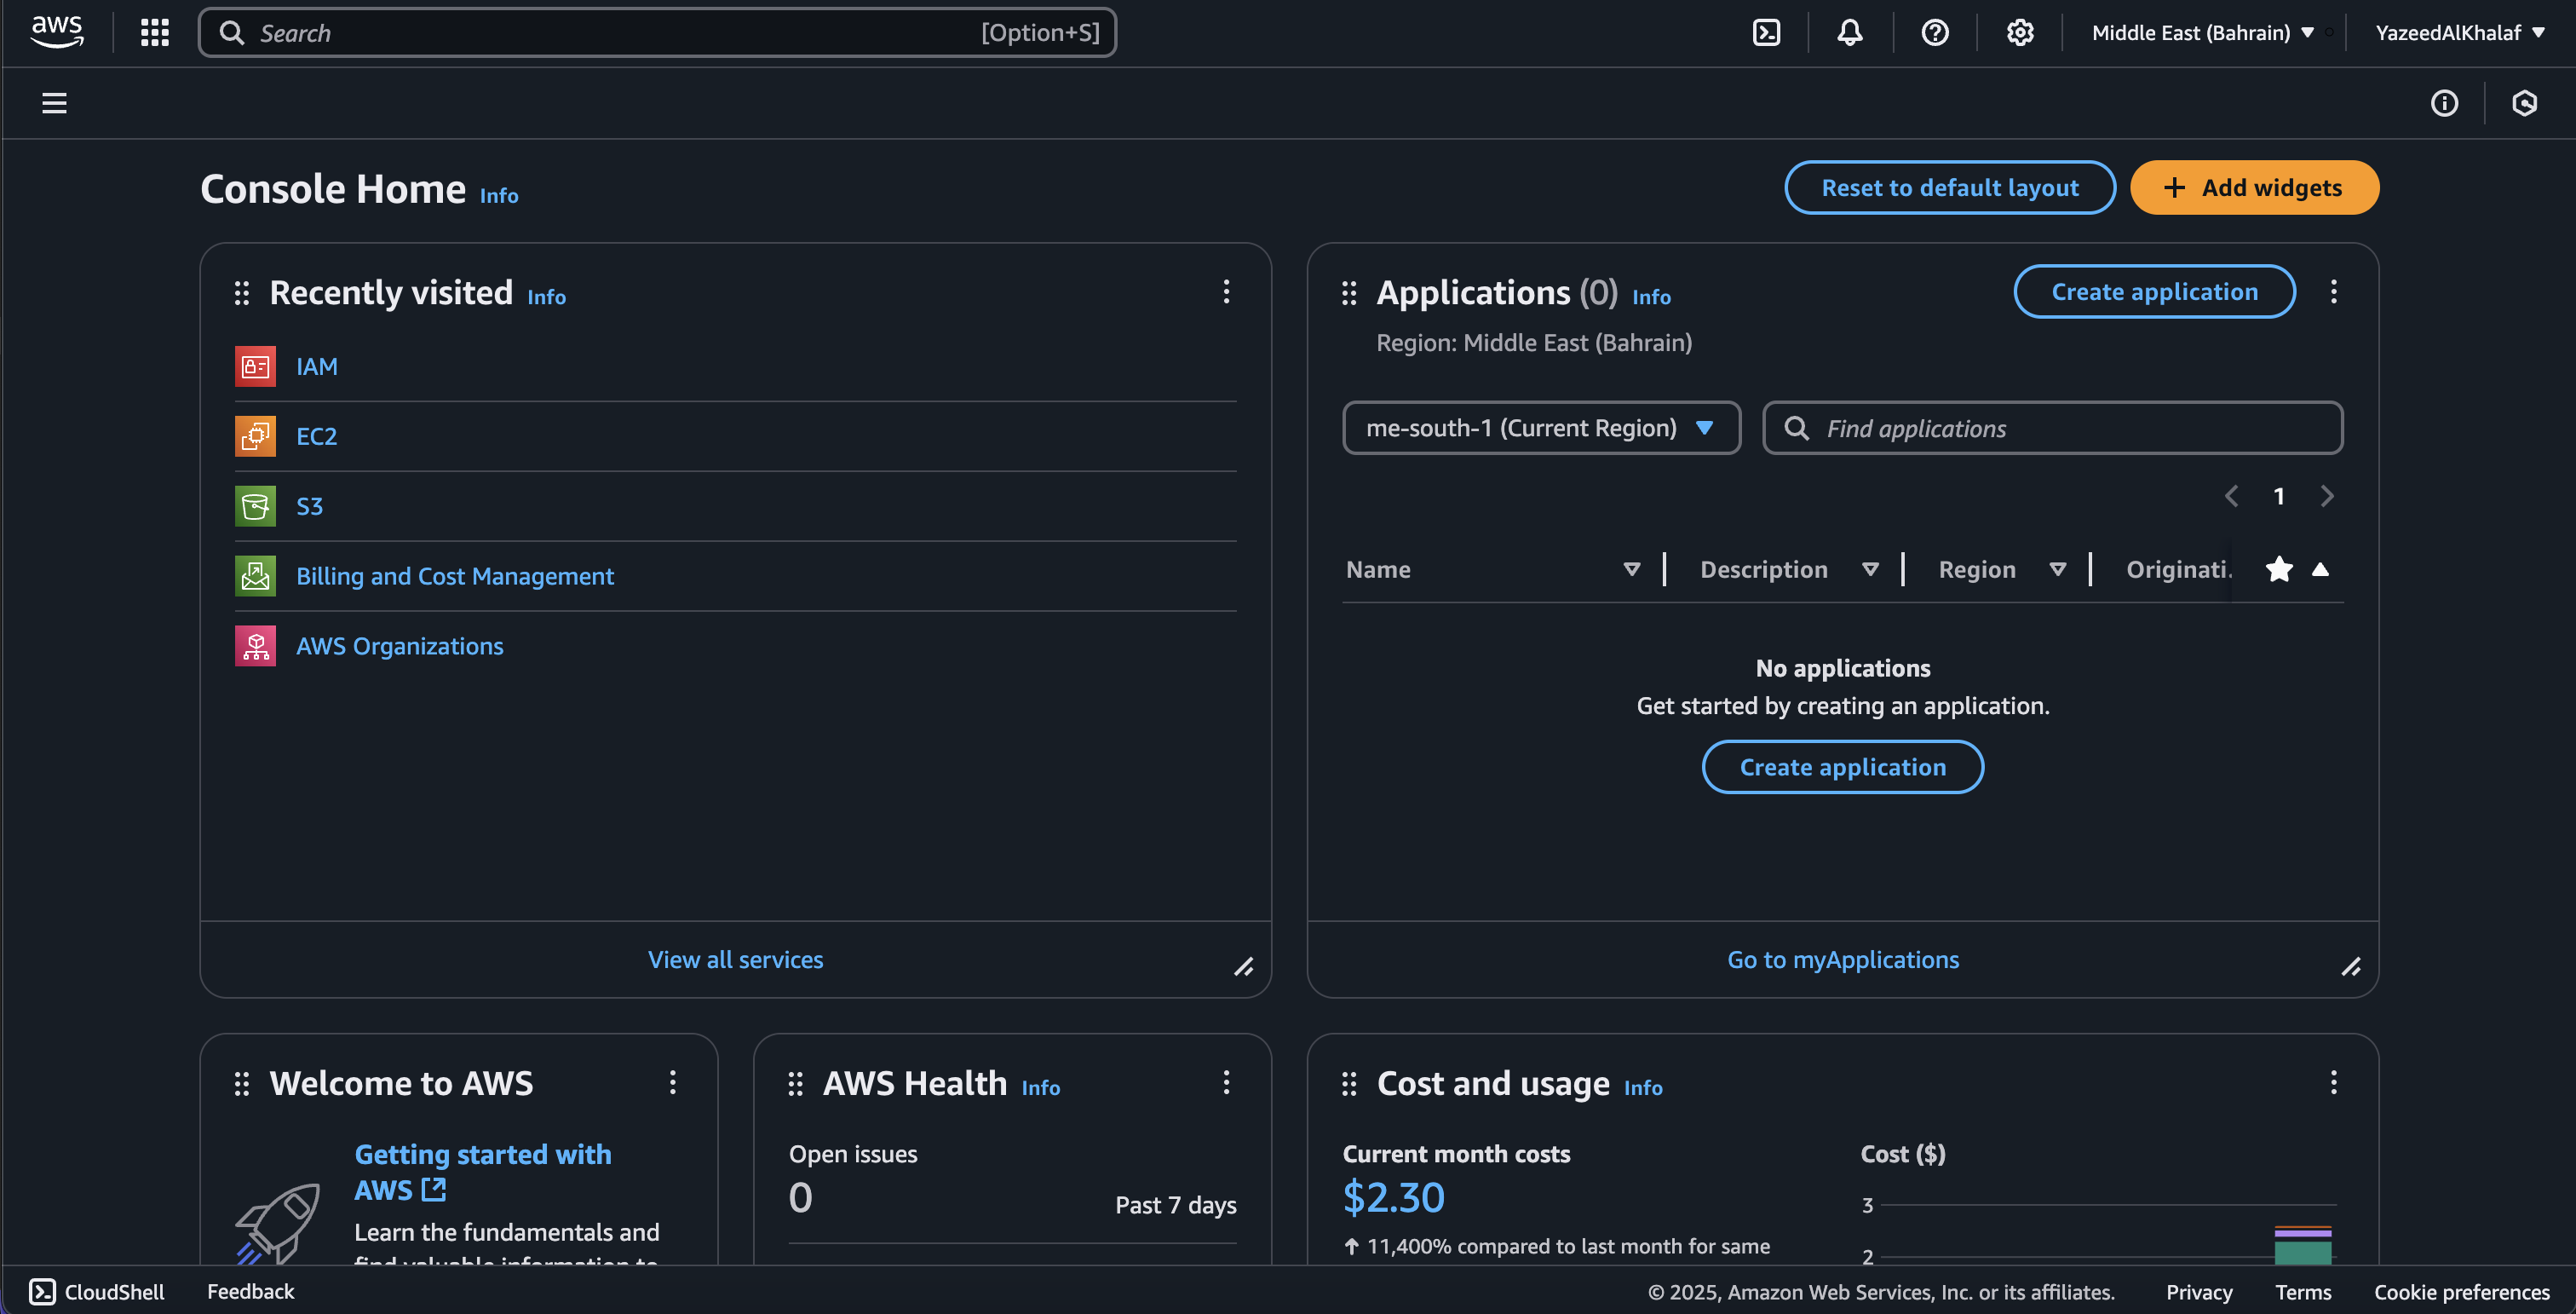
\includegraphics[width=0.95\textwidth]{aws-account.png}
    \caption{AWS Account Creation}
    \label{fig:aws-account}
\end{figure}

\begin{figure}[H]
    \centering
    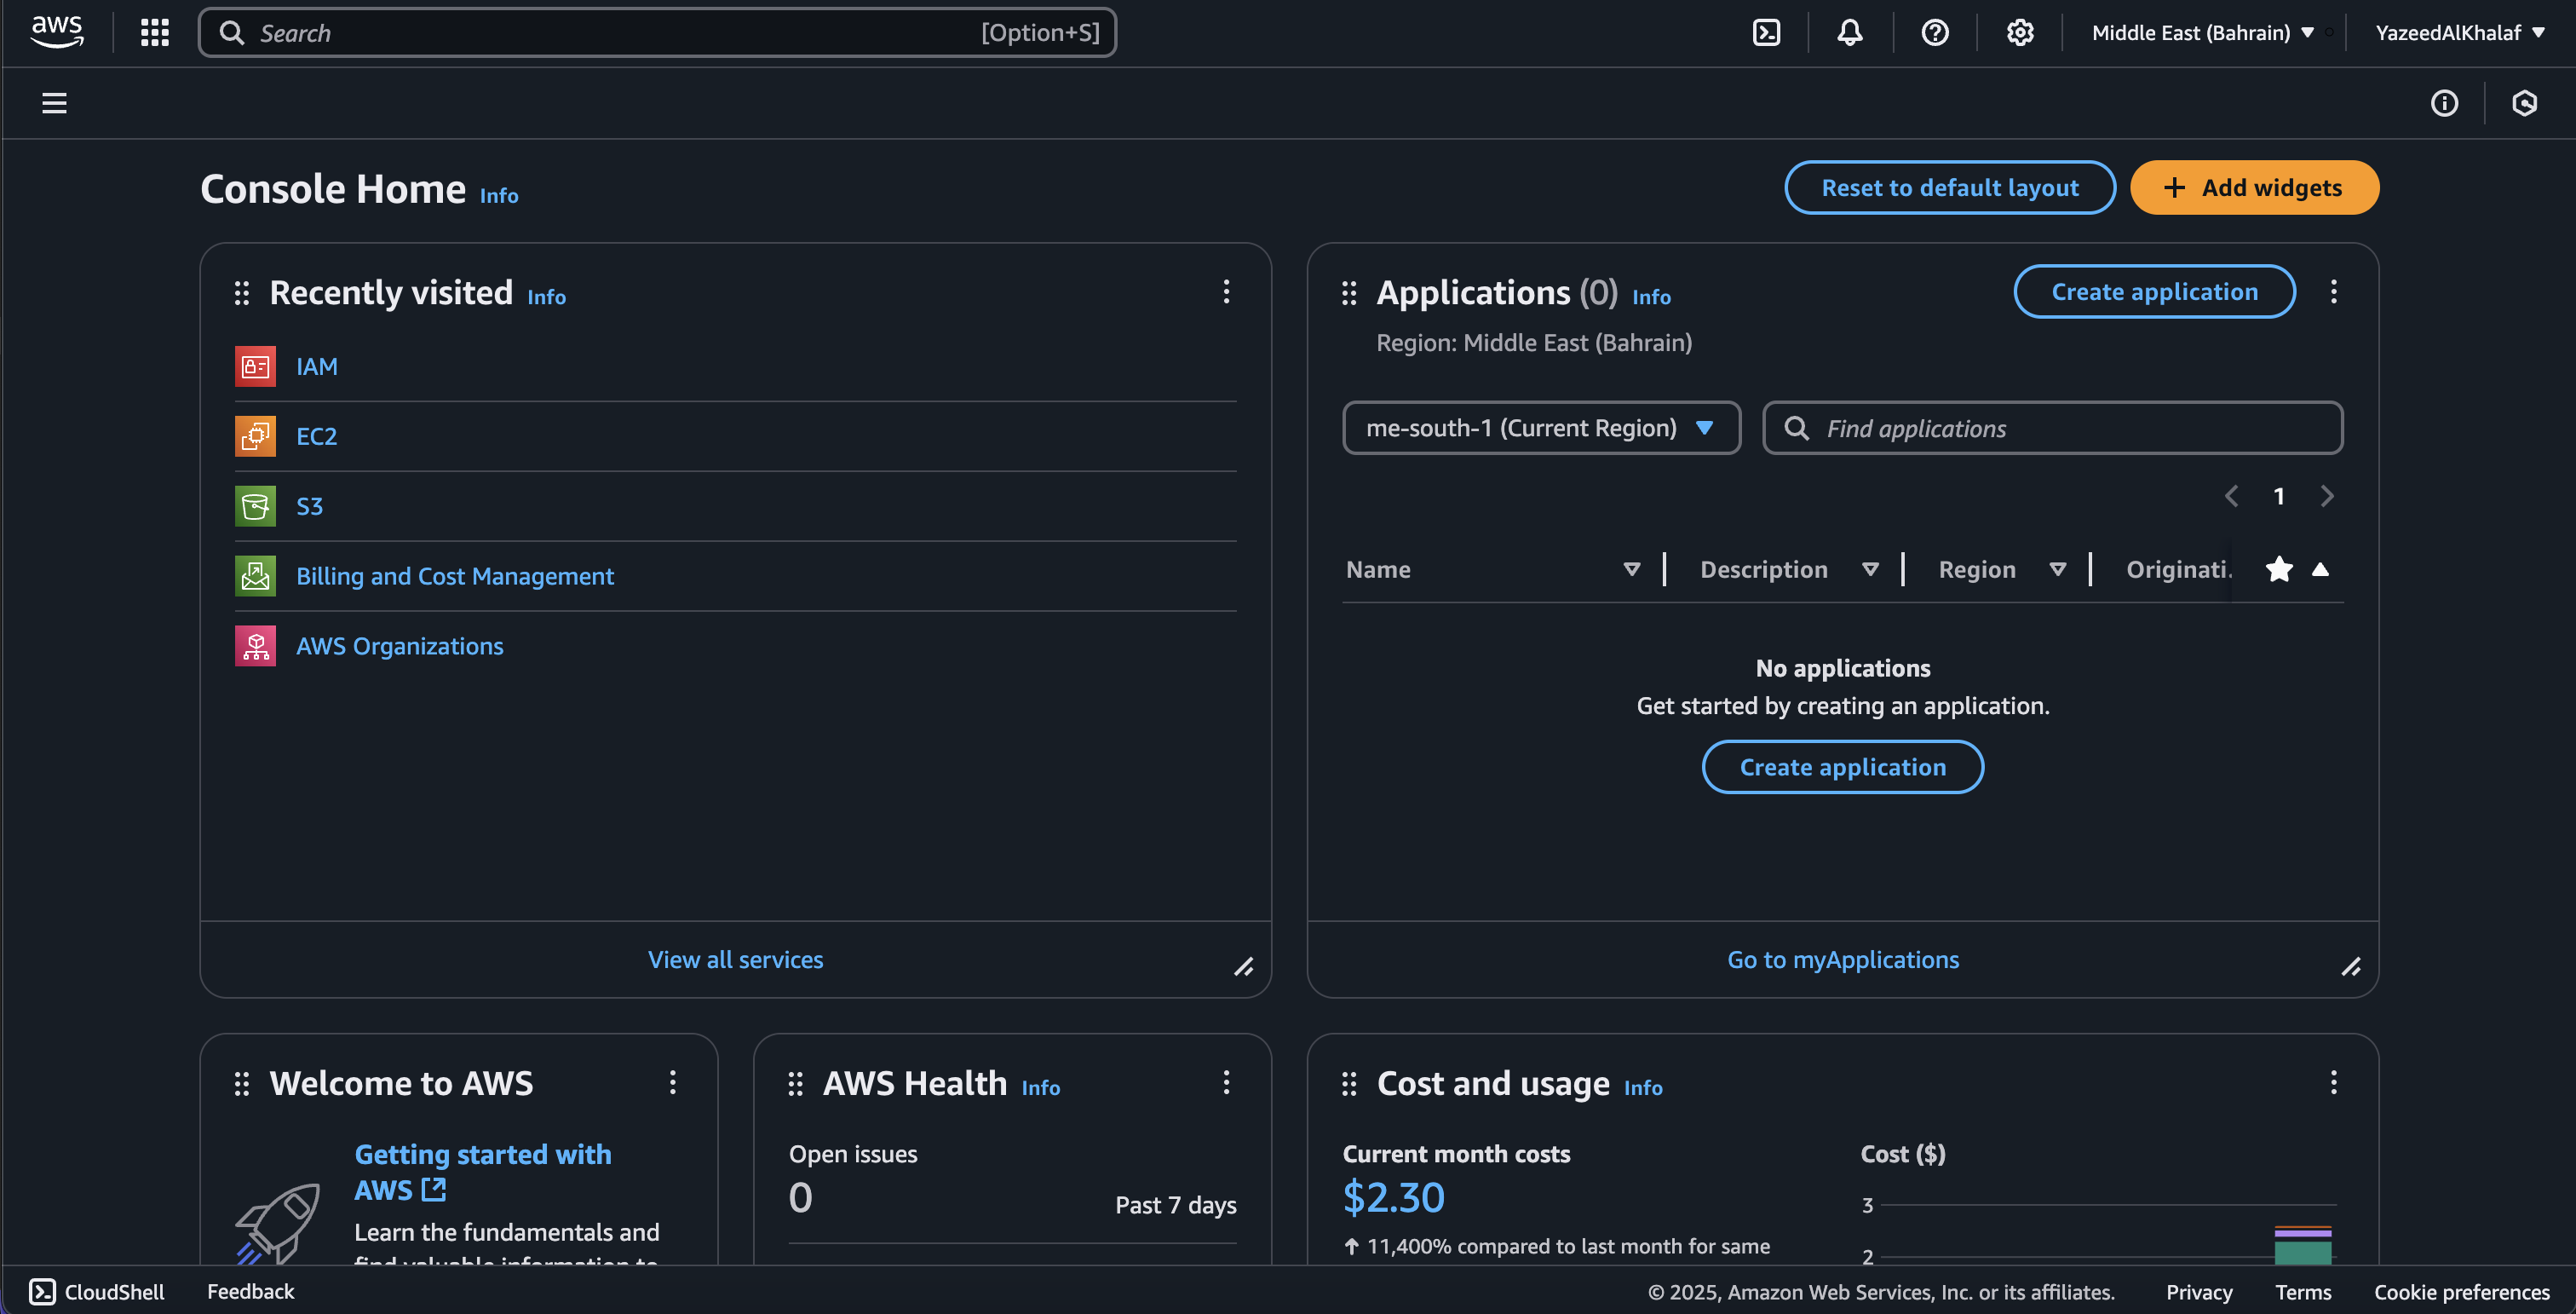
\includegraphics[width=0.95\textwidth]{aws-account.png}
    \caption{AWS Zero Spend Budget Configuration}
    \label{fig:aws-zero-spend-budget-config}
\end{figure}

\newpage

\section{Part B: Secure Your AWS Account}

\begin{figure}[H]
    \centering
    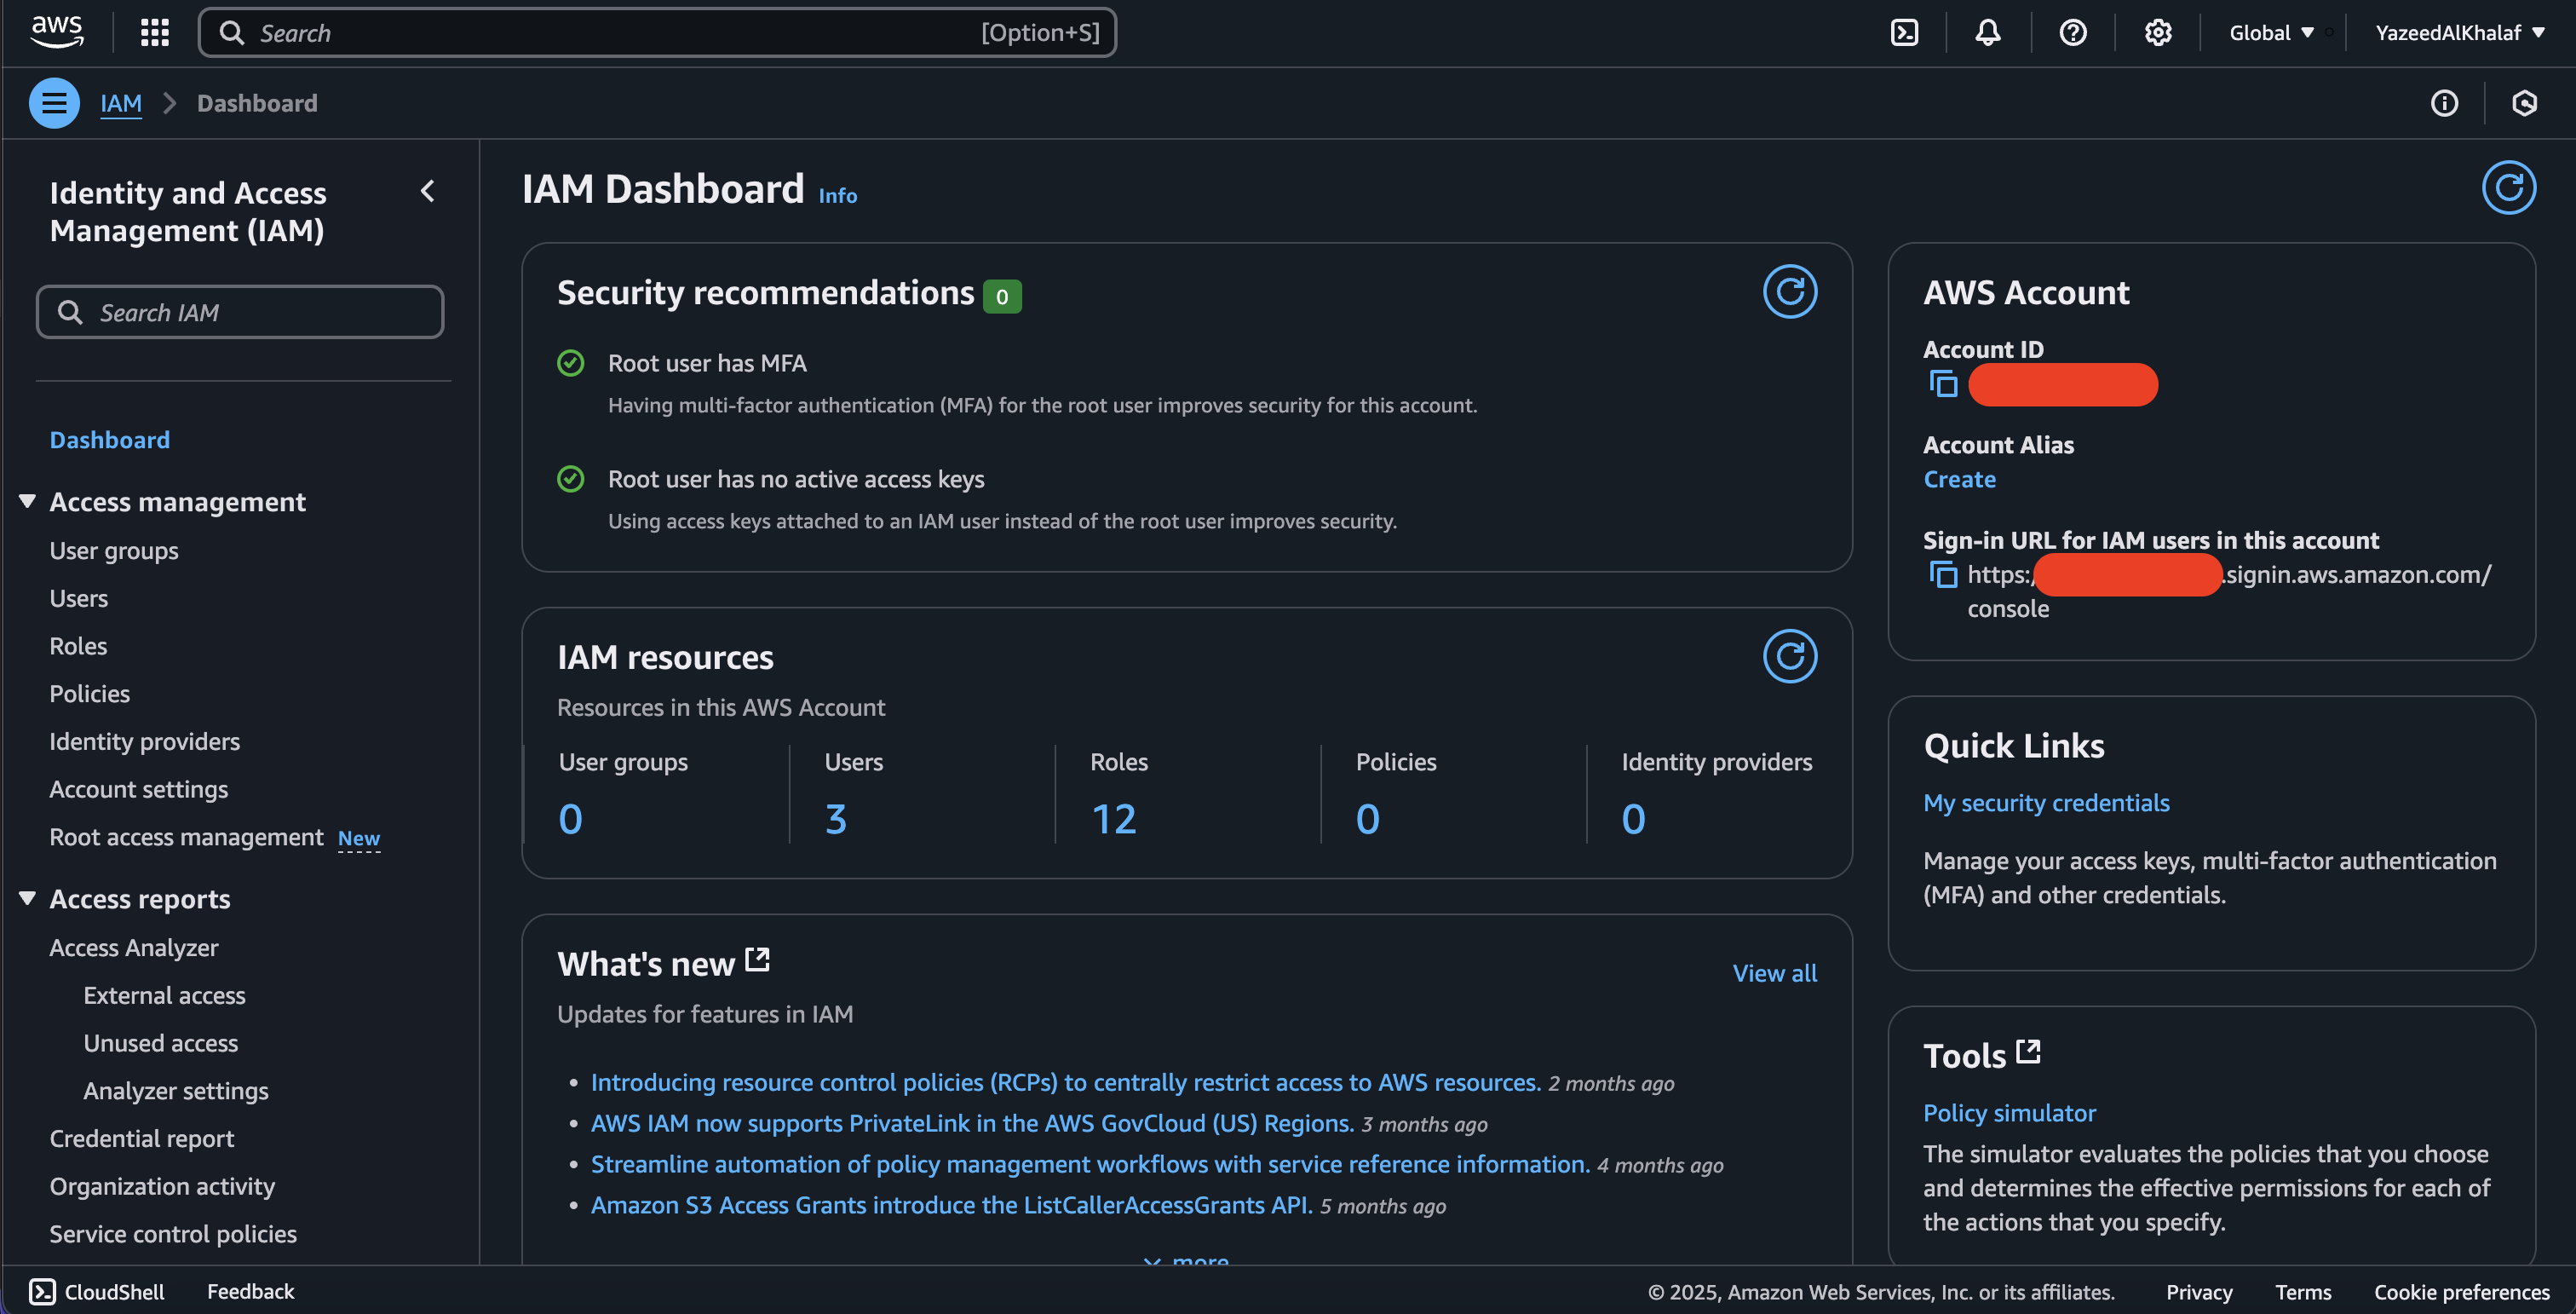
\includegraphics[width=0.95\textwidth]{secure-your-account.png}
    \caption{AWS Account Security Configuration}
    \label{fig:secure-account}
\end{figure}

\newpage

\section{Part C: Create IAM Account}

\begin{figure}[H]
    \centering
    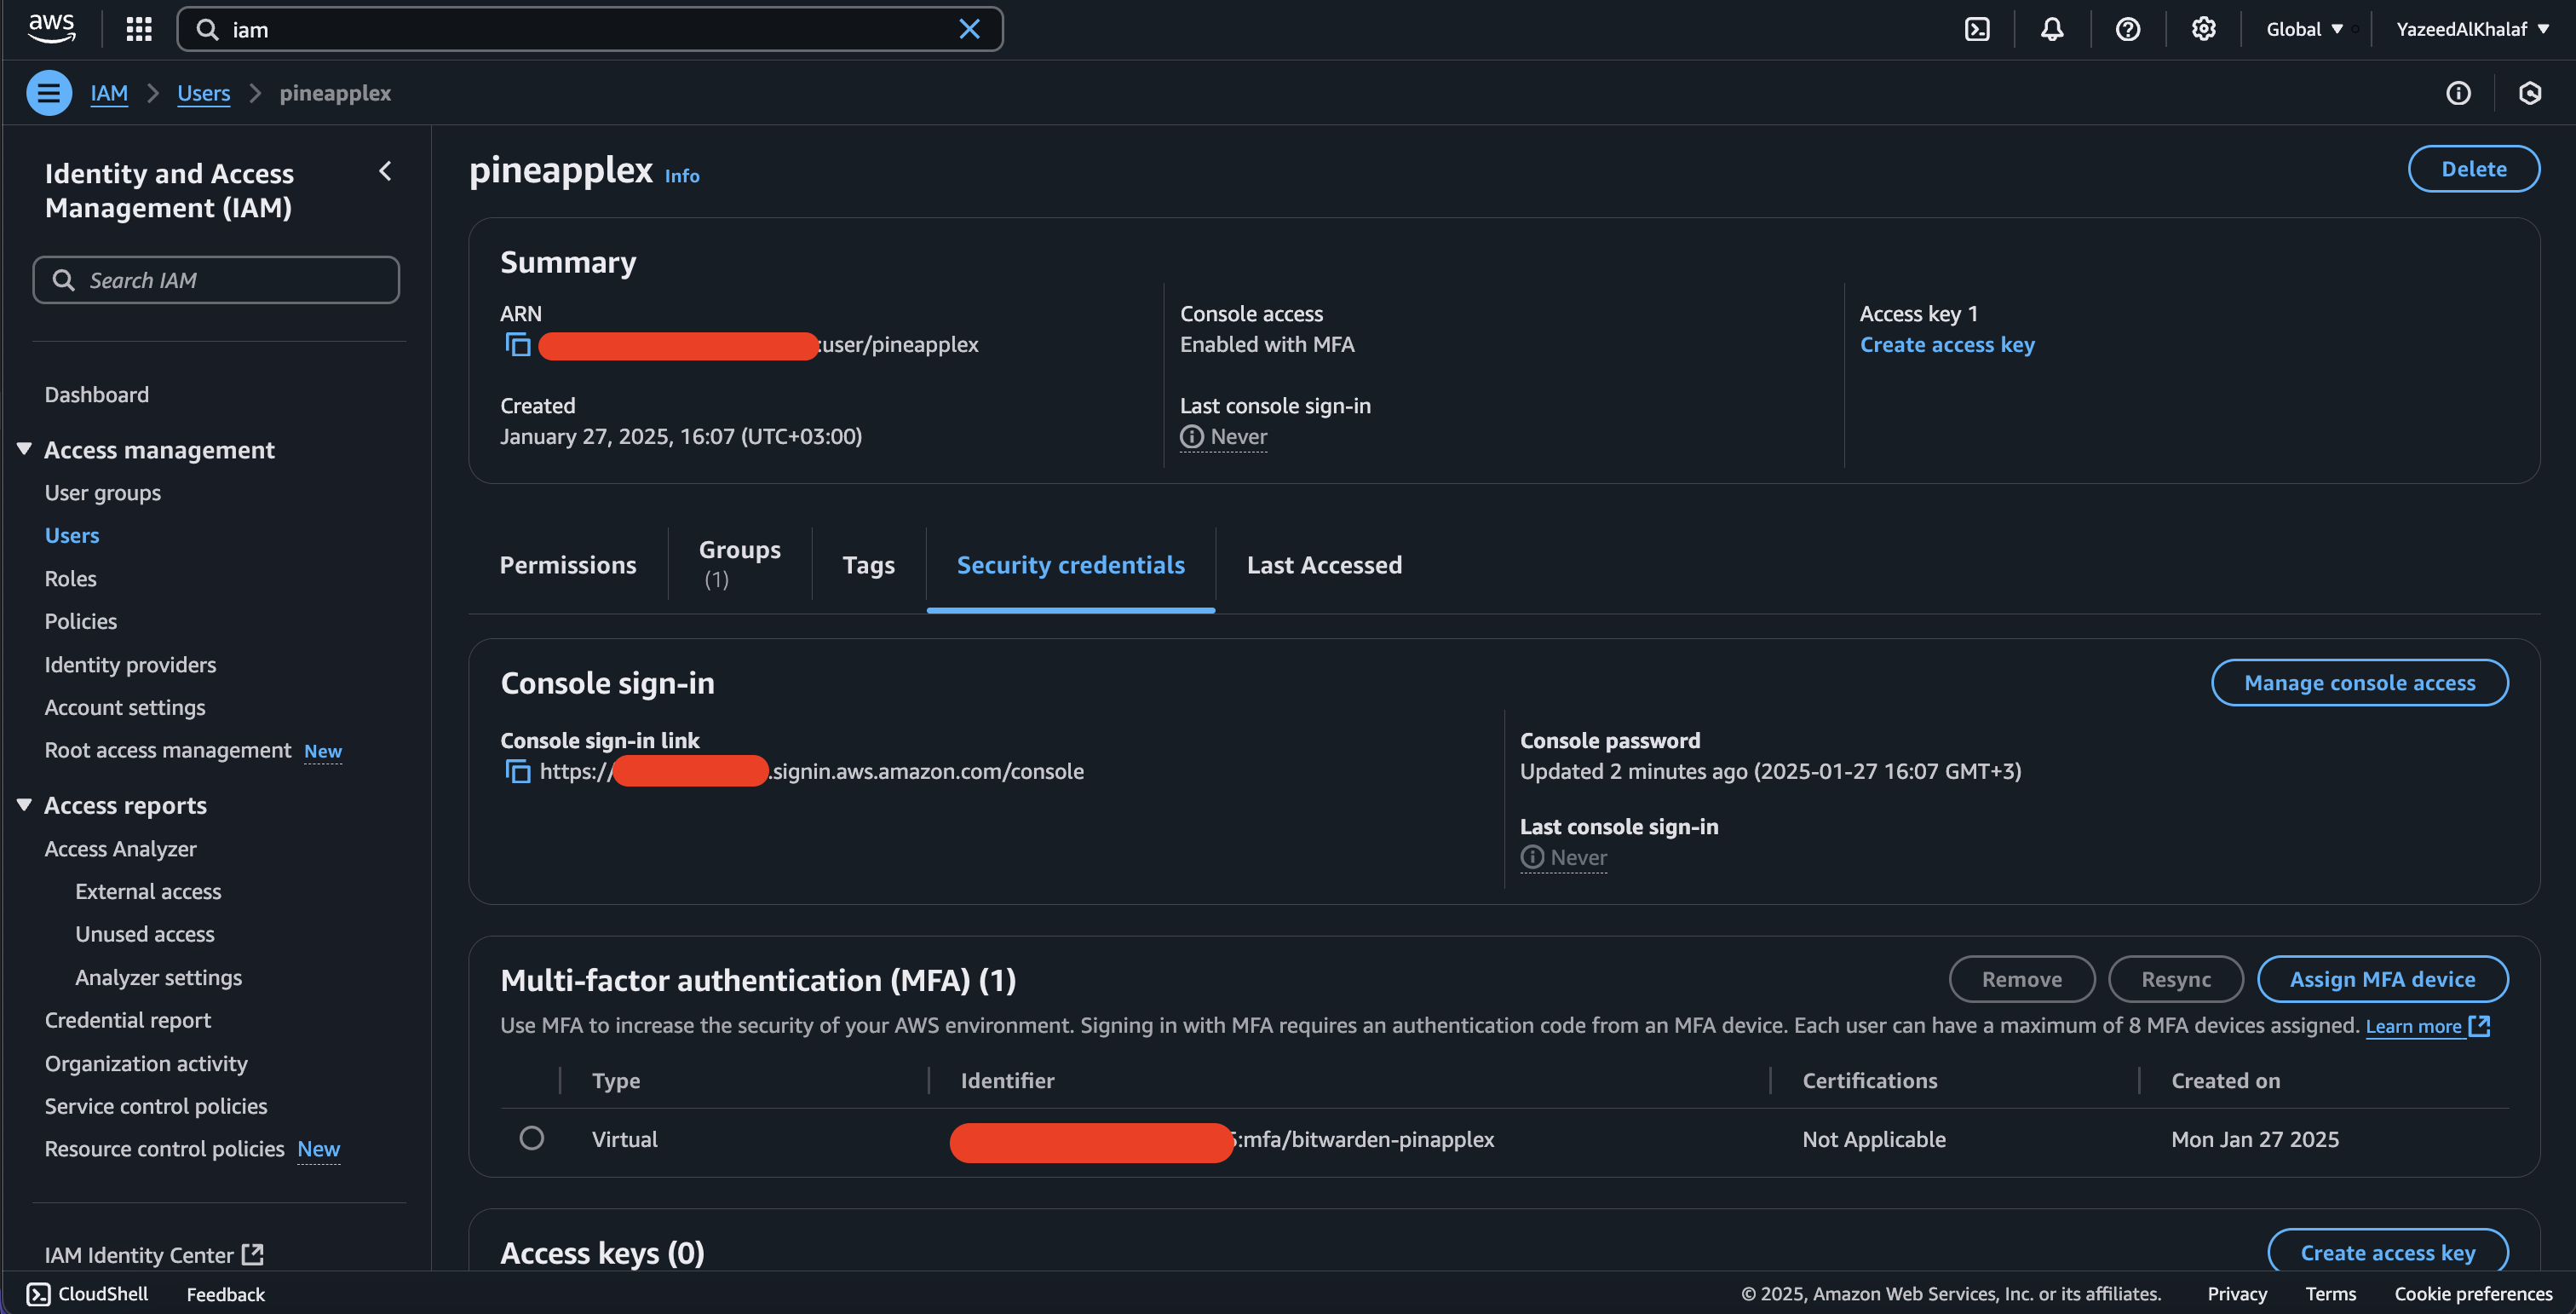
\includegraphics[width=0.95\textwidth]{iam-account.png}
    \caption{IAM Account Creation and Setup}
    \label{fig:iam-account}
\end{figure}

\newpage

\section{Part D: Create EC2 Instance and Security Groups}

\subsection{Launch EC2 Instance}

\begin{figure}[H]
    \centering
    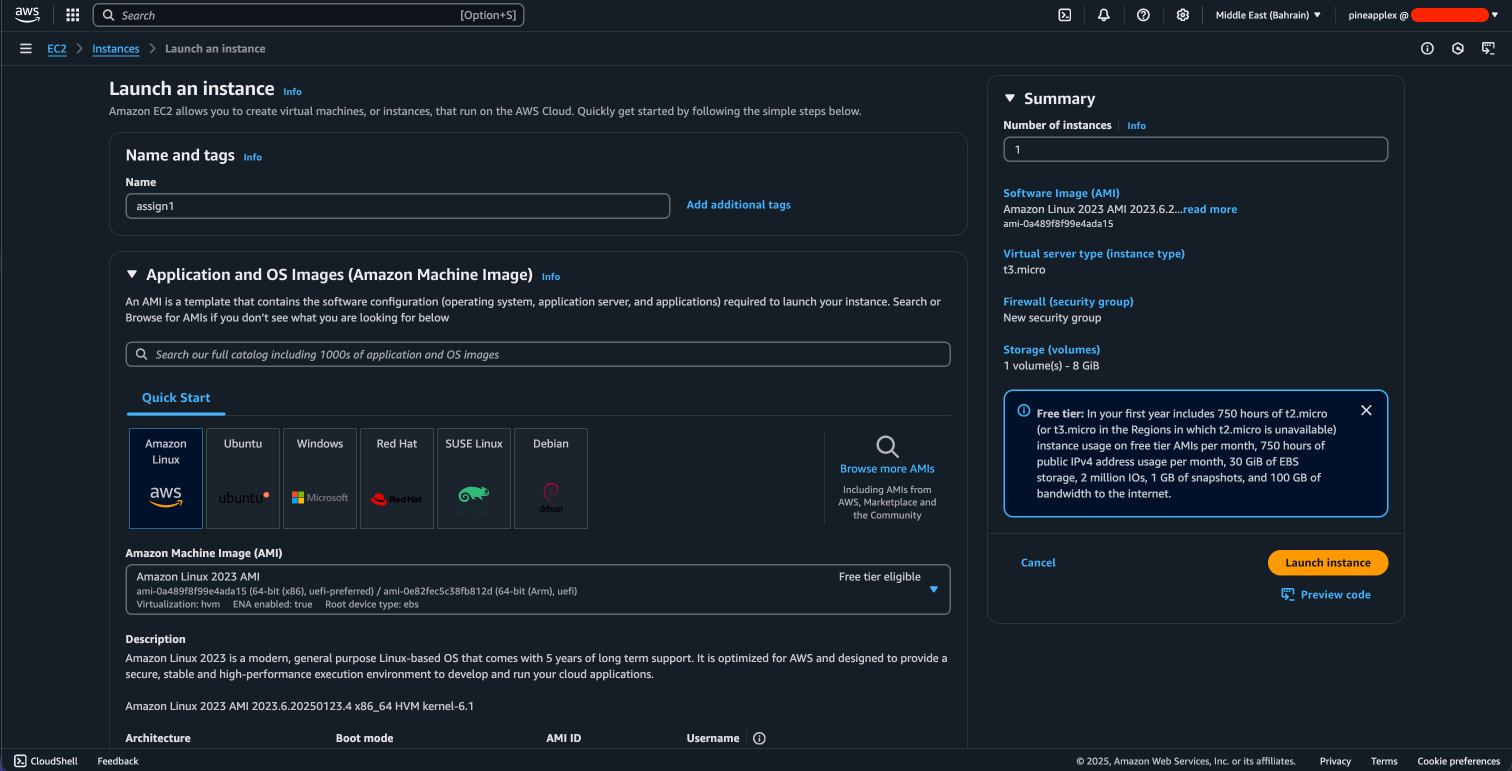
\includegraphics[width=0.95\textwidth]{launch-instance-1.png}
    \caption{EC2 Instance Launch Configuration - Instance Type Selection}
    \label{fig:ec2-launch1}
\end{figure}

\begin{figure}[H]
    \centering
    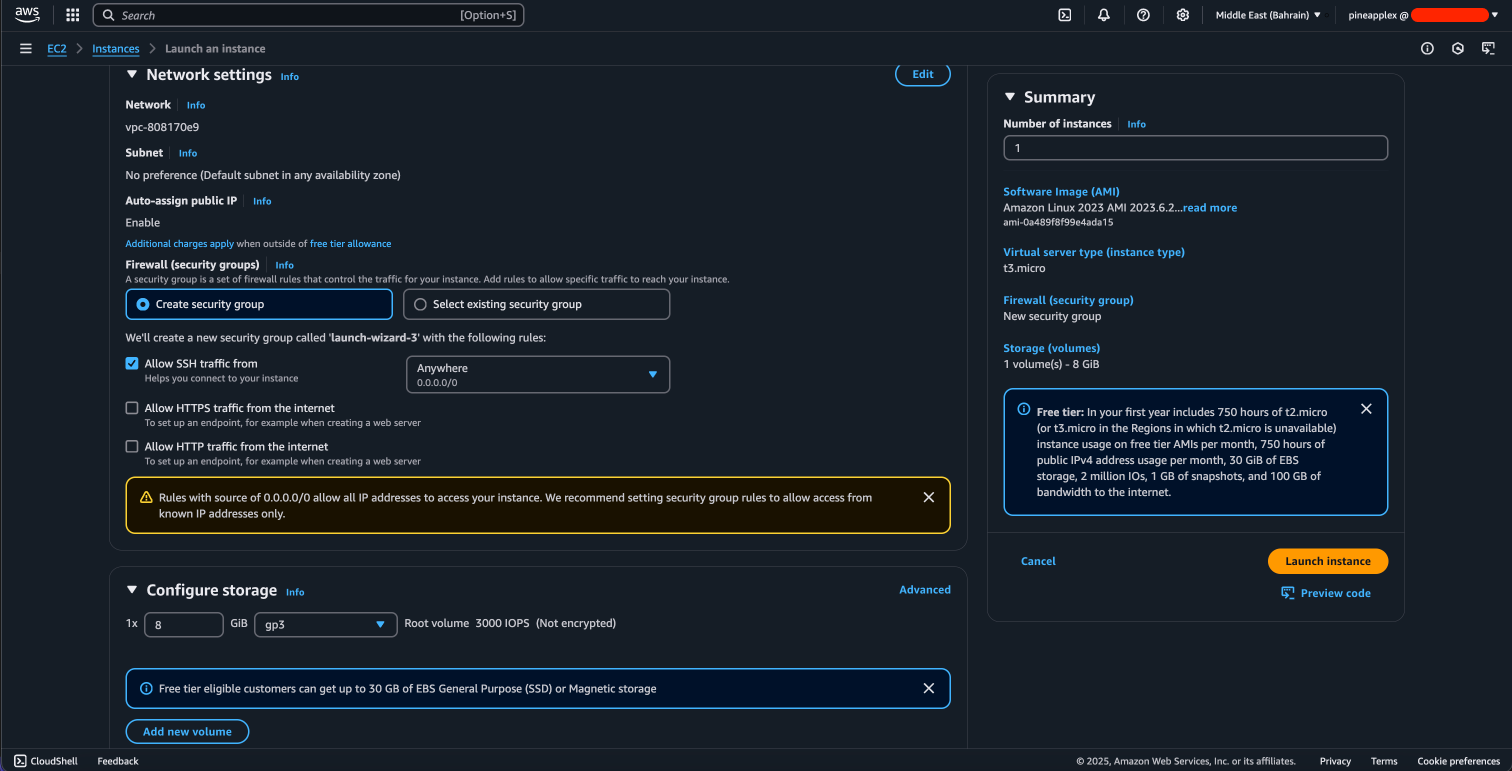
\includegraphics[width=0.95\textwidth]{launch-instance-2.png}
    \caption{EC2 Instance Launch Configuration - Network Settings}
    \label{fig:ec2-launch2}
\end{figure}

\begin{figure}[H]
    \centering
    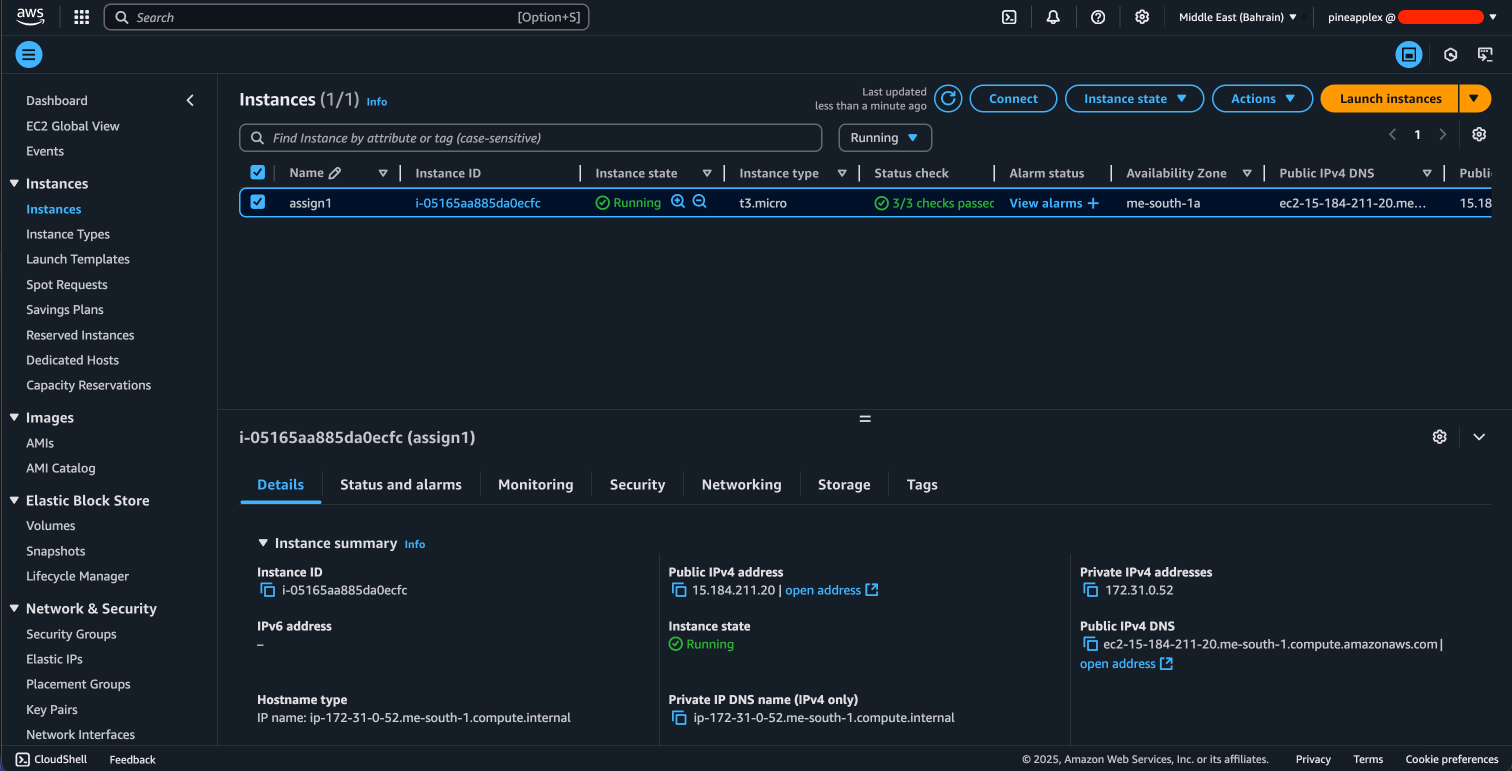
\includegraphics[width=0.95\textwidth]{launch-instance-3.png}
    \caption{EC2 Instance Launch Configuration - Successfully Launched}
    \label{fig:ec2-launch3}
\end{figure}

\newpage

\subsection{Create Security Groups}

\begin{figure}[H]
    \centering
    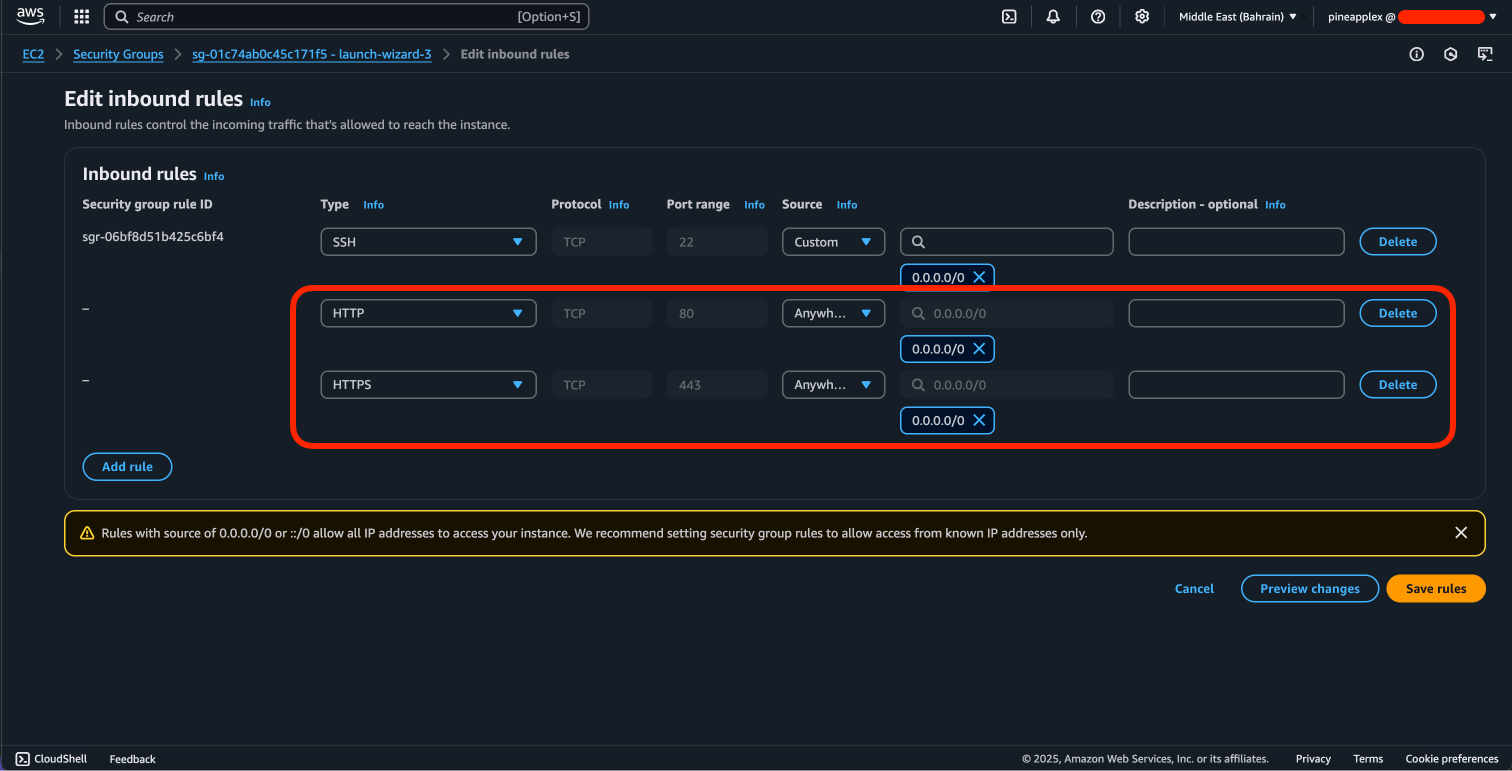
\includegraphics[width=0.95\textwidth]{security-groups-1.png}
    \caption{Security Group Configuration - Inbound Rules Addition}
    \label{fig:security1}
\end{figure}

\begin{figure}[H]
    \centering
    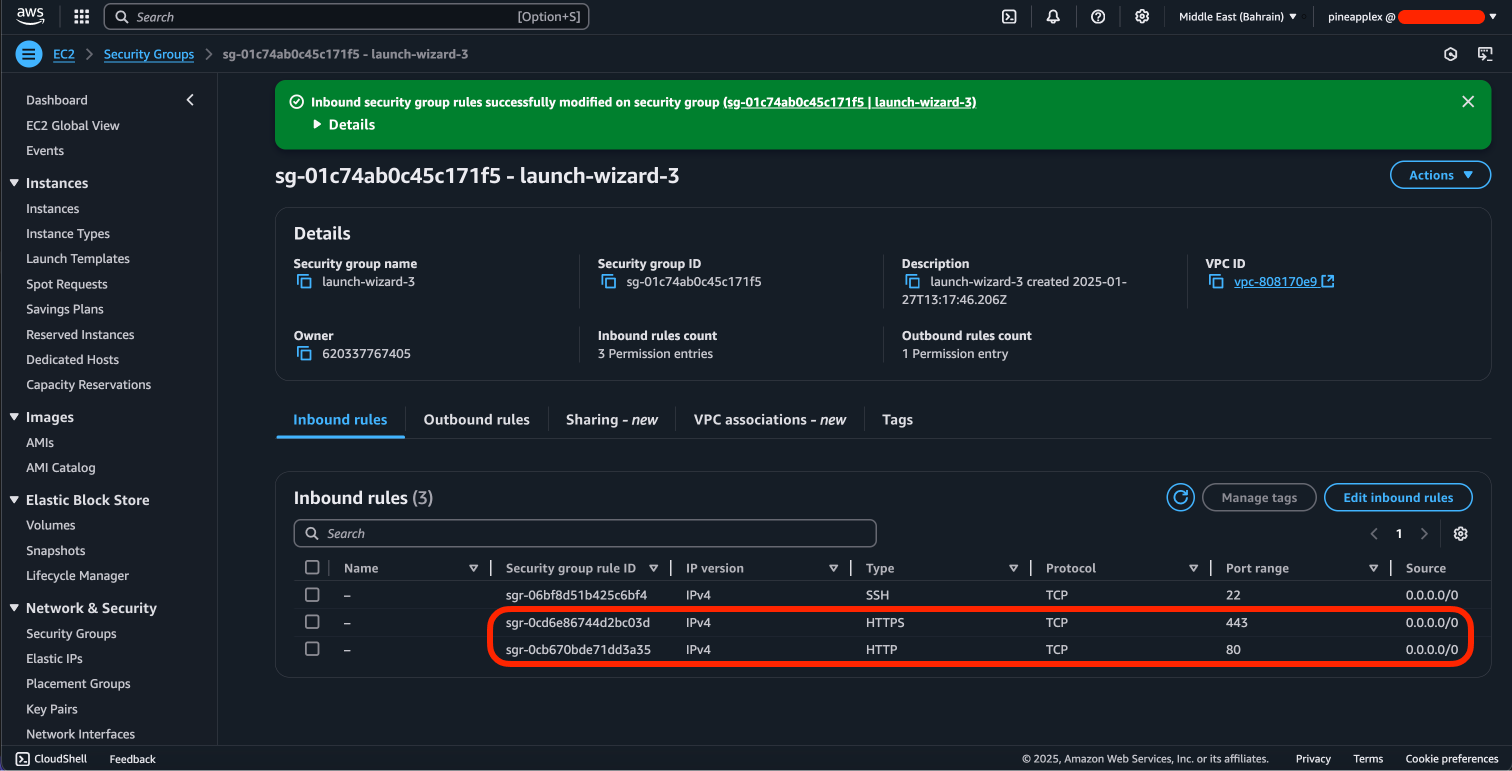
\includegraphics[width=0.95\textwidth]{security-groups-2.png}
    \caption{Security Group Configuration - Outbound Rules Verification}
    \label{fig:security2}
\end{figure}

\newpage

\subsection{Configure Elastic IP}

\begin{figure}[H]
    \centering
    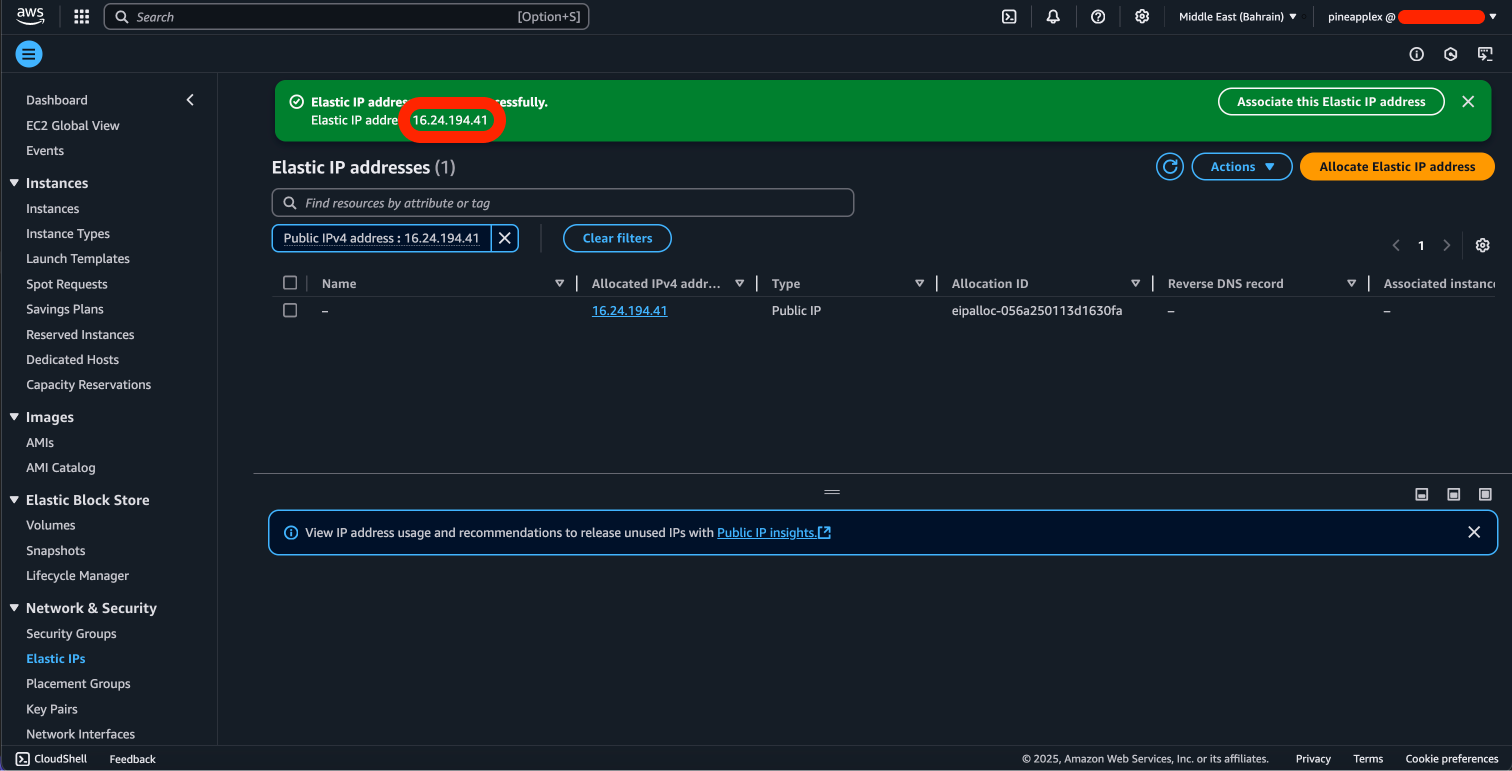
\includegraphics[width=0.95\textwidth]{elastic-ip-1.png}
    \caption{Elastic IP Configuration - Allocation}
    \label{fig:elastic1}
\end{figure}

\begin{figure}[H]
    \centering
    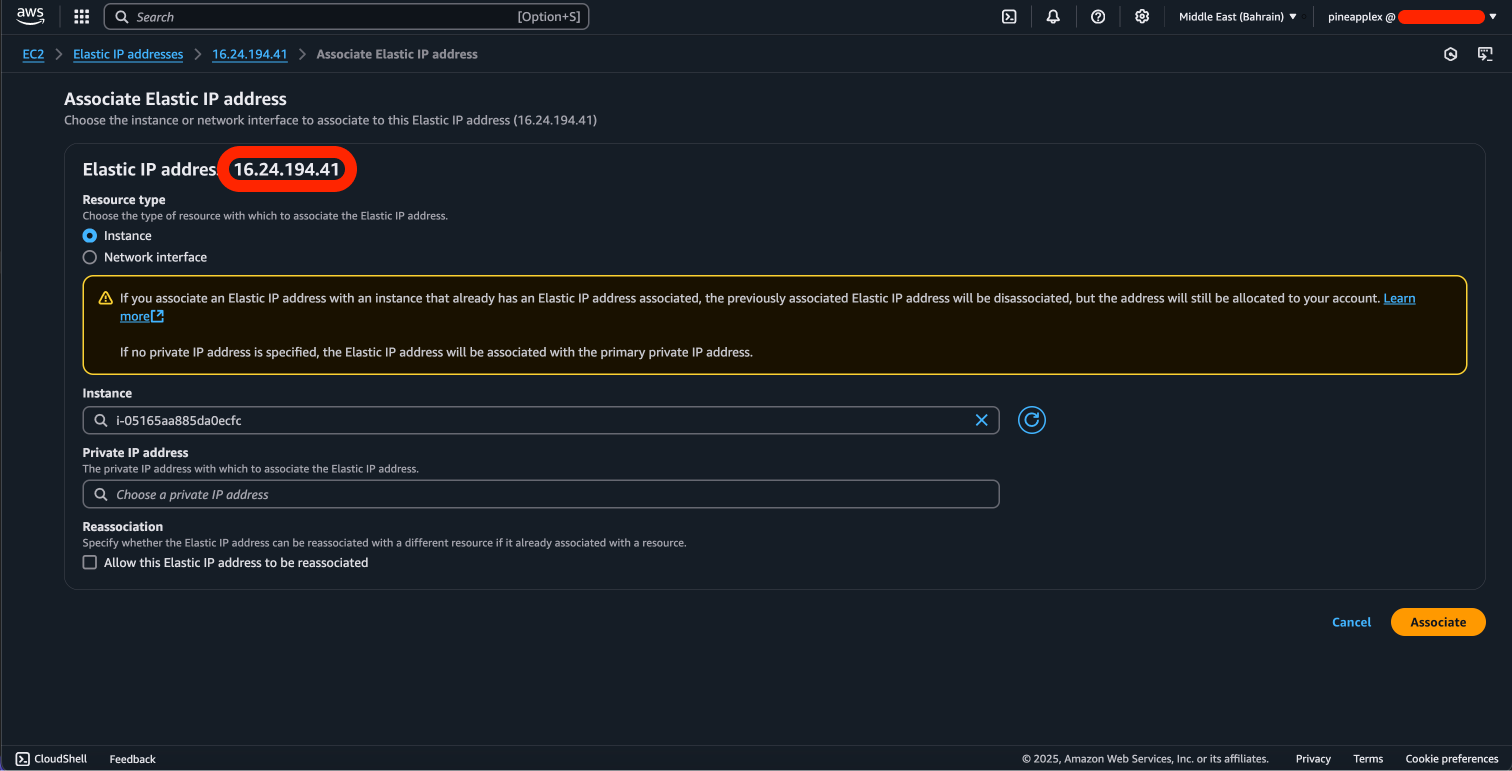
\includegraphics[width=0.95\textwidth]{elastic-ip-2.png}
    \caption{Elastic IP Configuration - Association}
    \label{fig:elastic2}
\end{figure}

\begin{figure}[H]
    \centering
    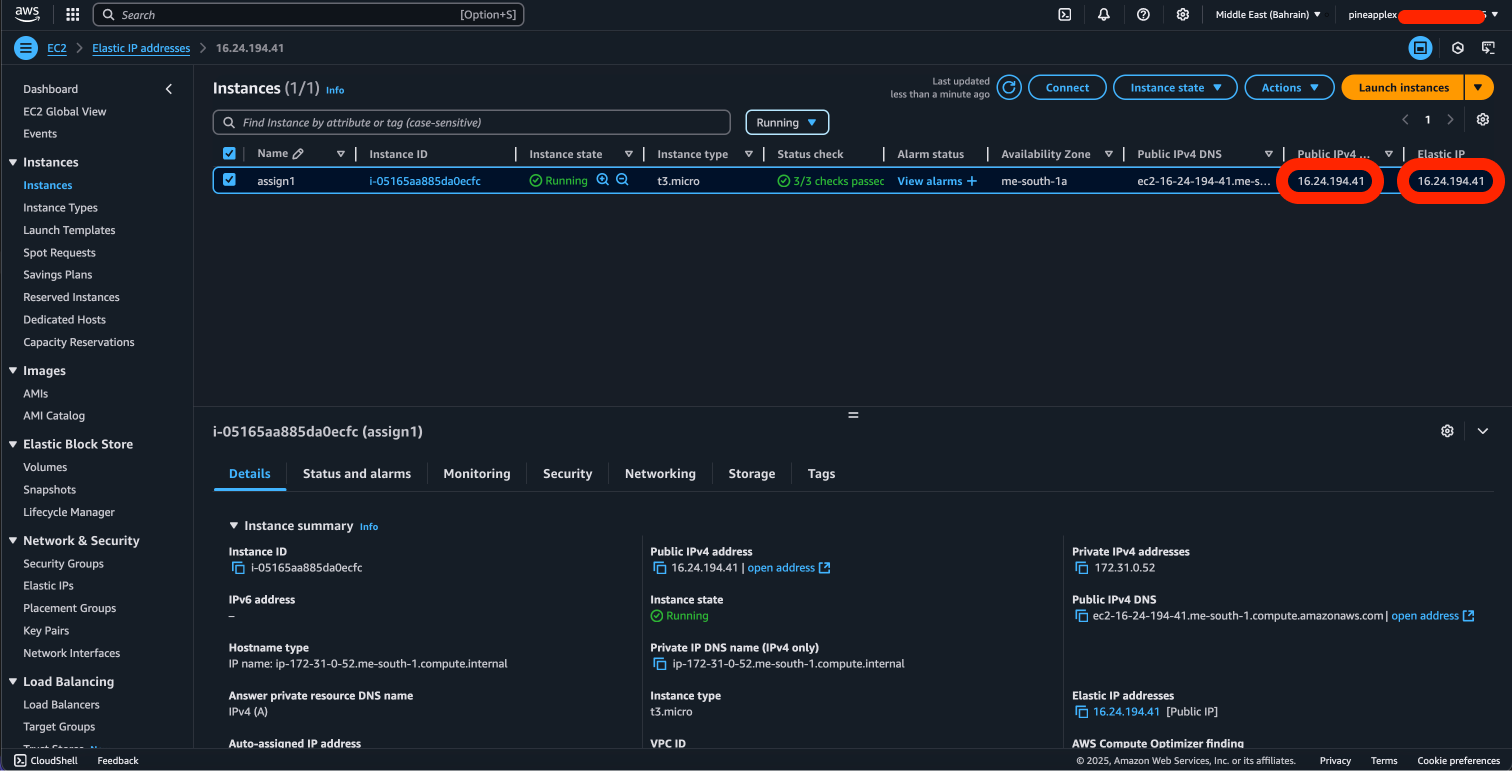
\includegraphics[width=0.95\textwidth]{elastic-ip-3.png}
    \caption{Elastic IP Configuration - Verification}
    \label{fig:elastic3}
\end{figure}

\newpage

\section{Part E: Install a LAMP web server on Amazon Linux 2023}

\begin{figure}[H]
    \centering
    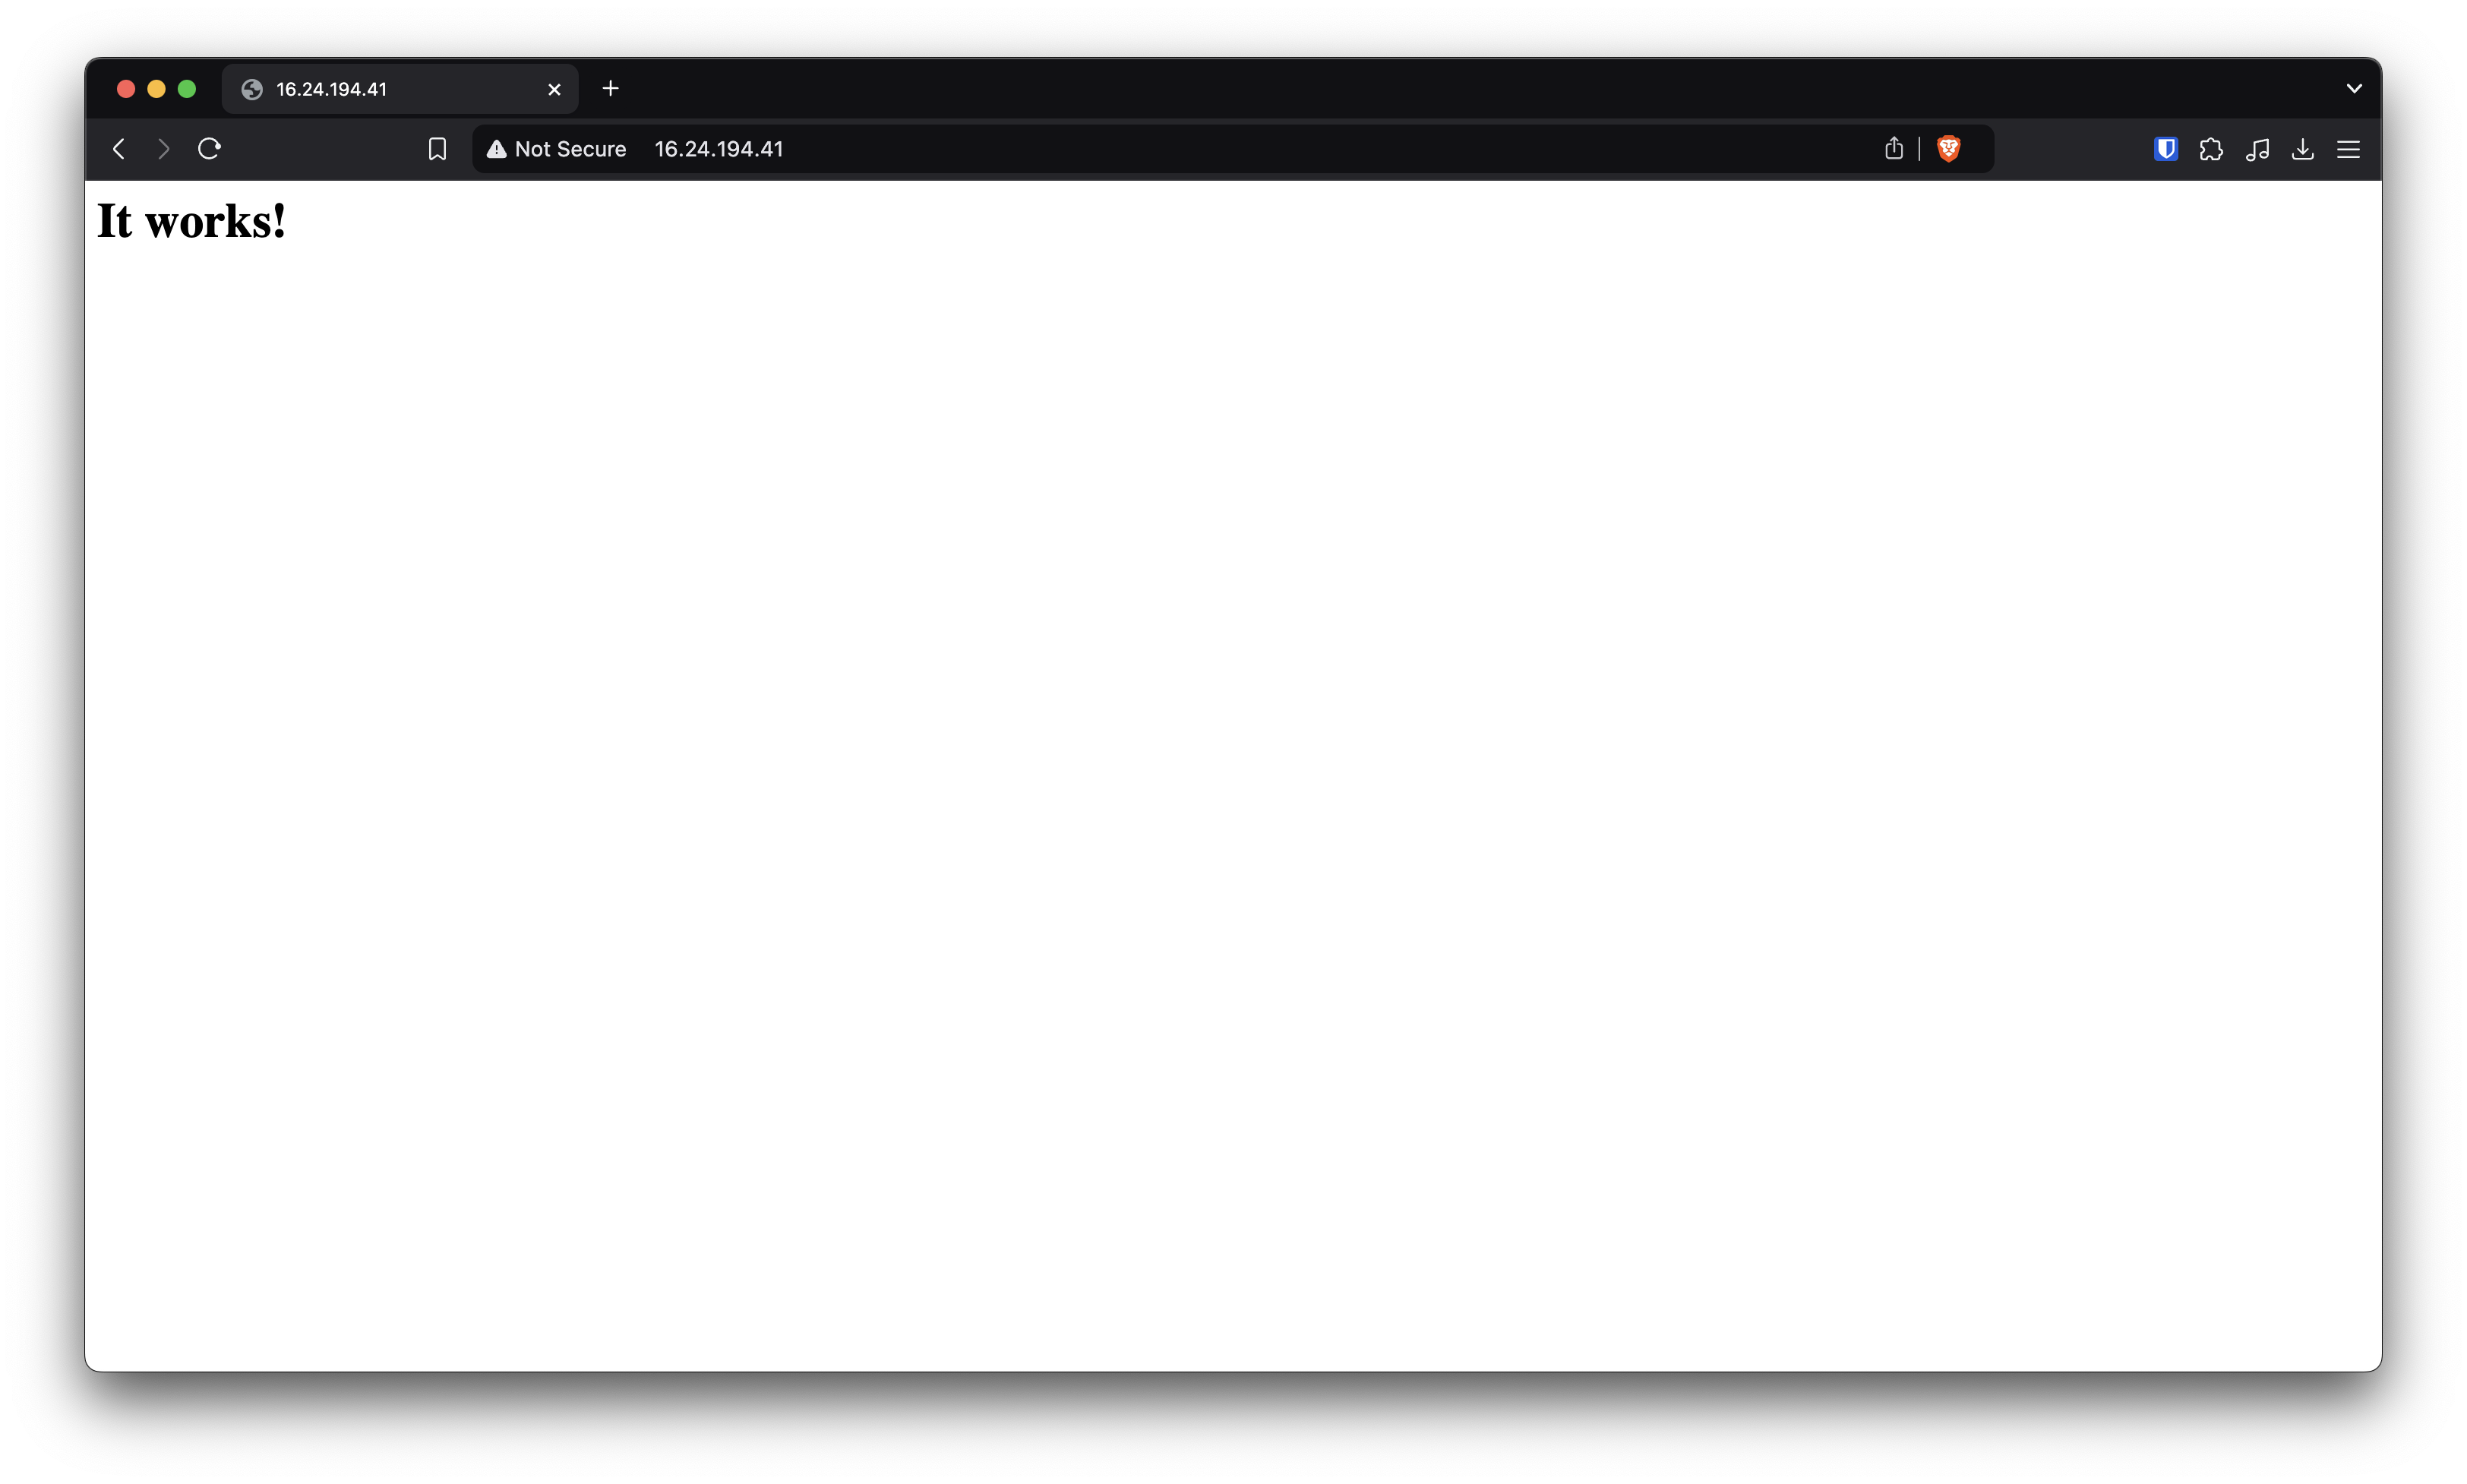
\includegraphics[width=0.95\textwidth]{lamp-server-1.png}
    \caption{LAMP Web Server - Successfully Installed}
    \label{fig:lamp1}
\end{figure}

\begin{figure}[H]
    \centering
    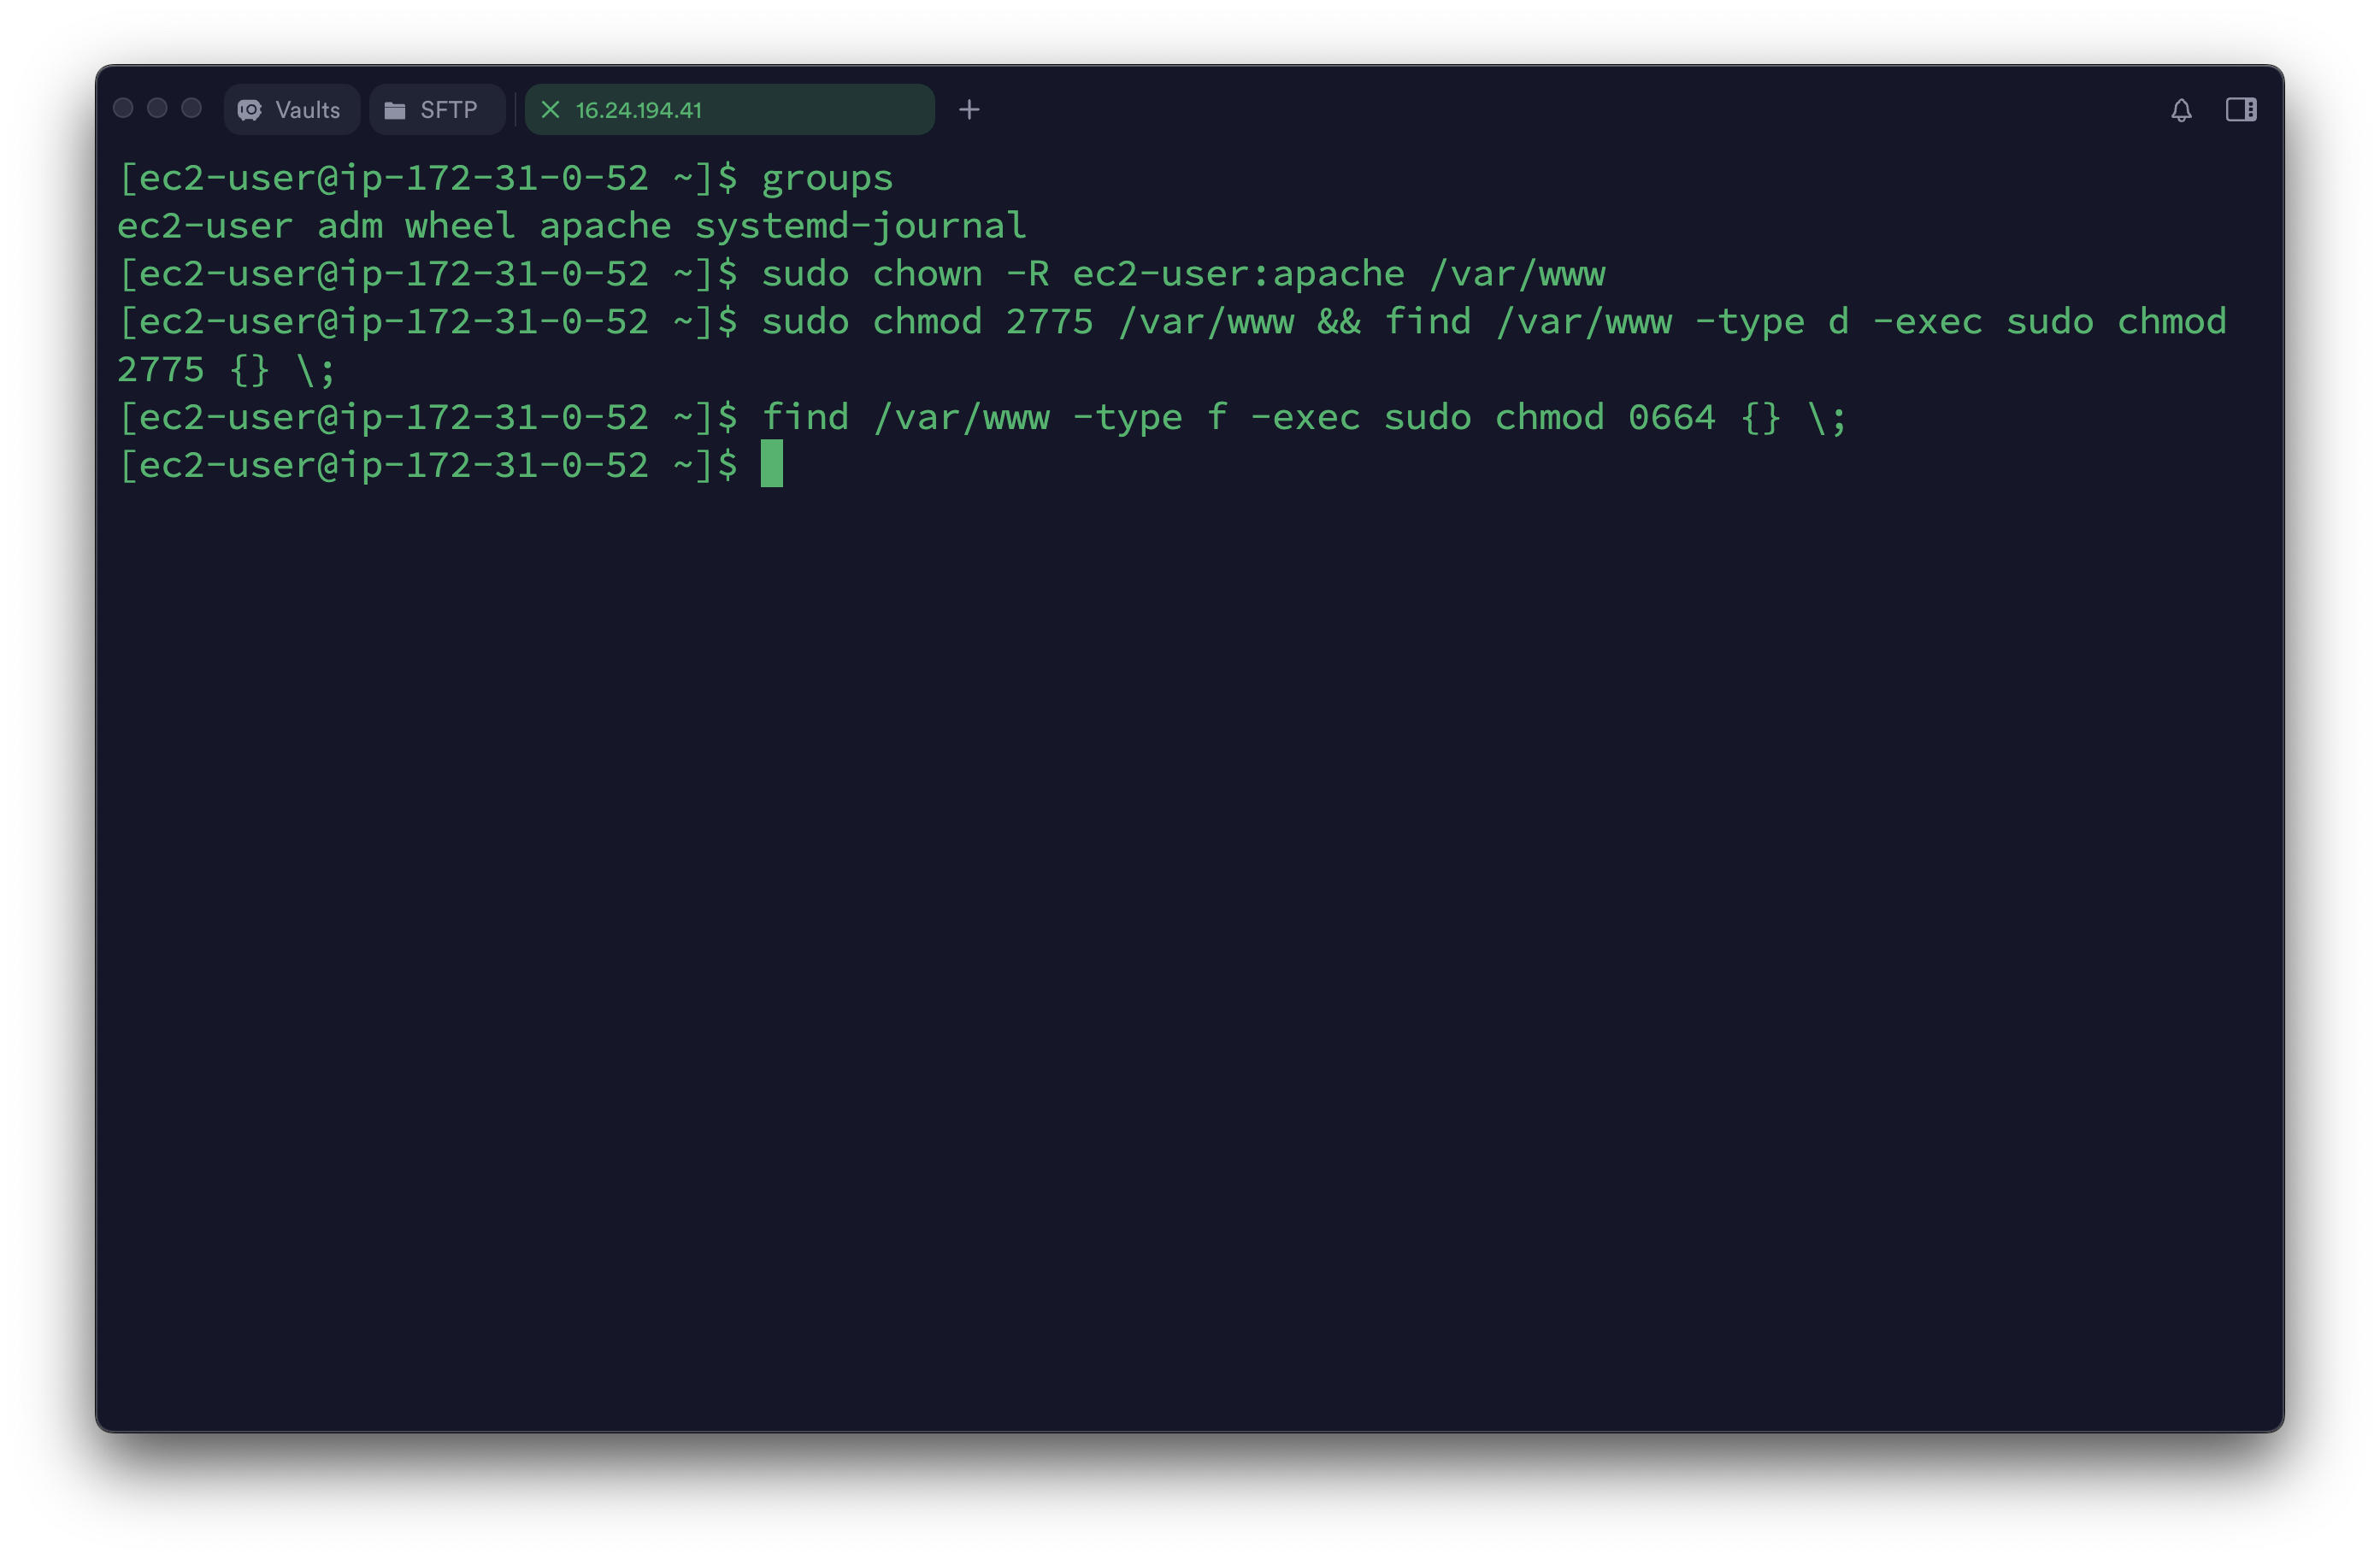
\includegraphics[width=0.95\textwidth]{lamp-server-2.png}
    \caption{LAMP Web Server - Adding ec2-user to apache group with other security practices}
    \label{fig:lamp2}
\end{figure}

\begin{figure}[H]
    \centering
    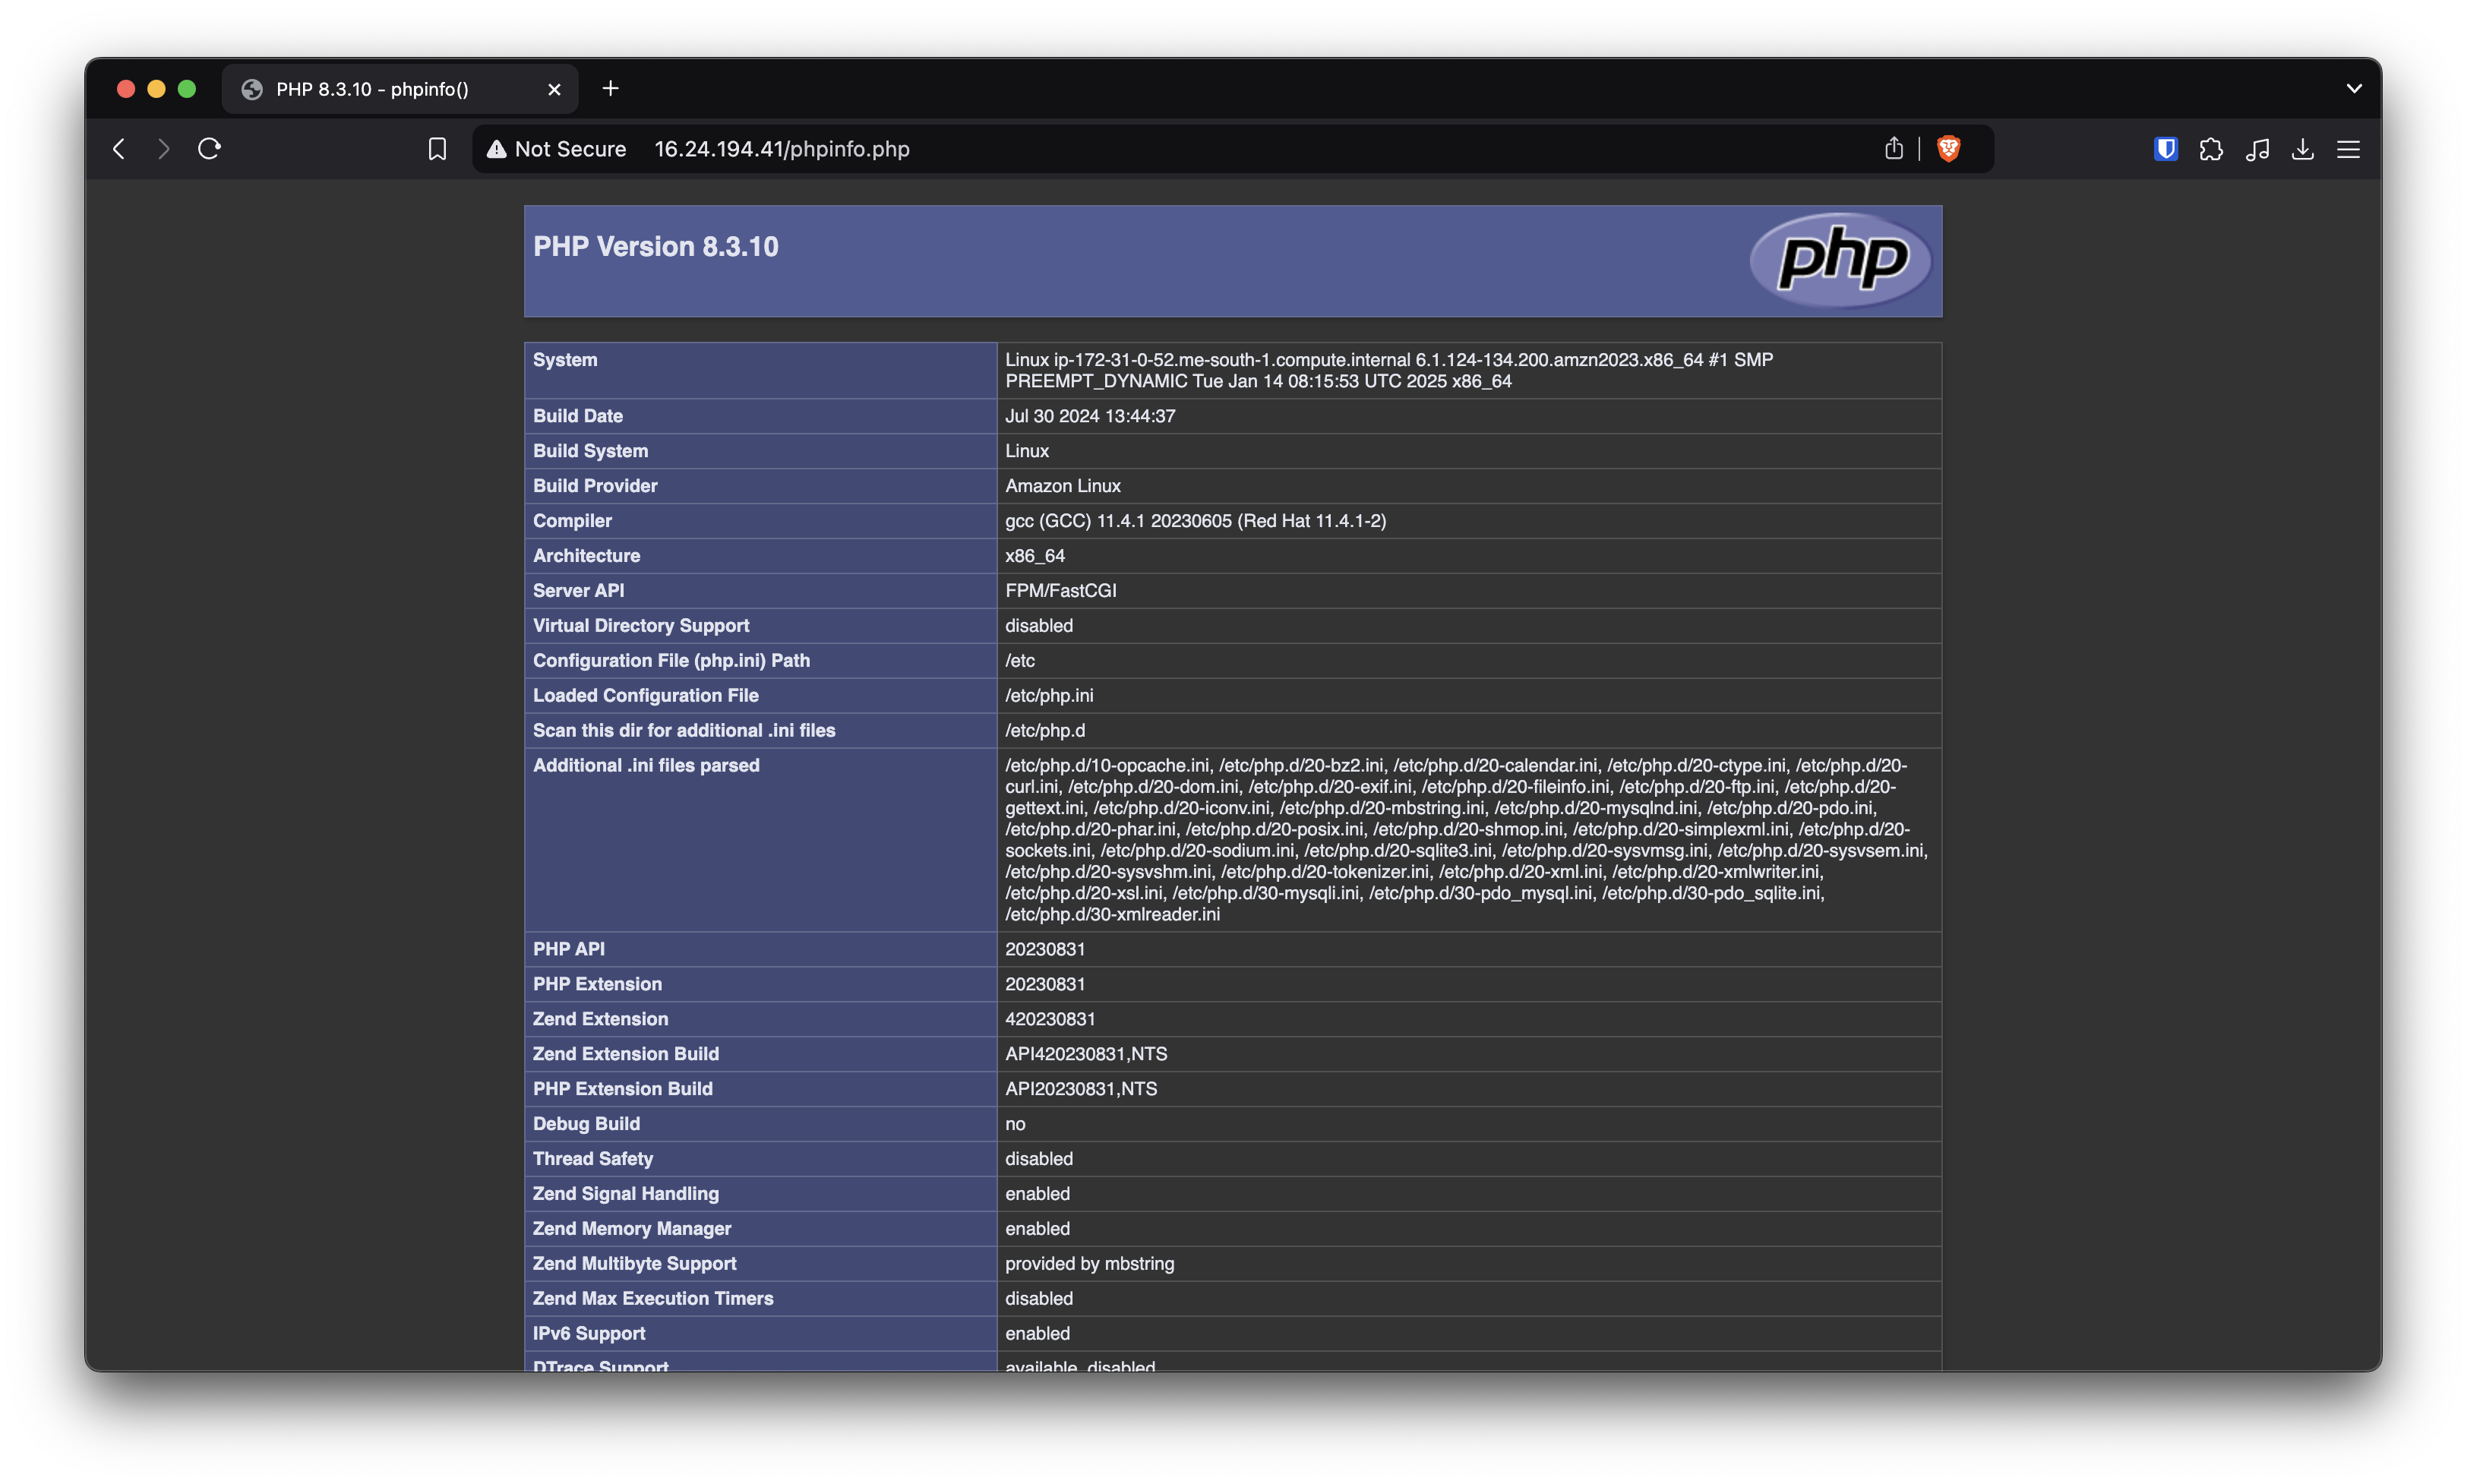
\includegraphics[width=0.95\textwidth]{lamp-server-3.png}
    \caption{LAMP Web Server - PHP Info Page}
    \label{fig:lamp3}
\end{figure}

\begin{figure}[H]
    \centering
    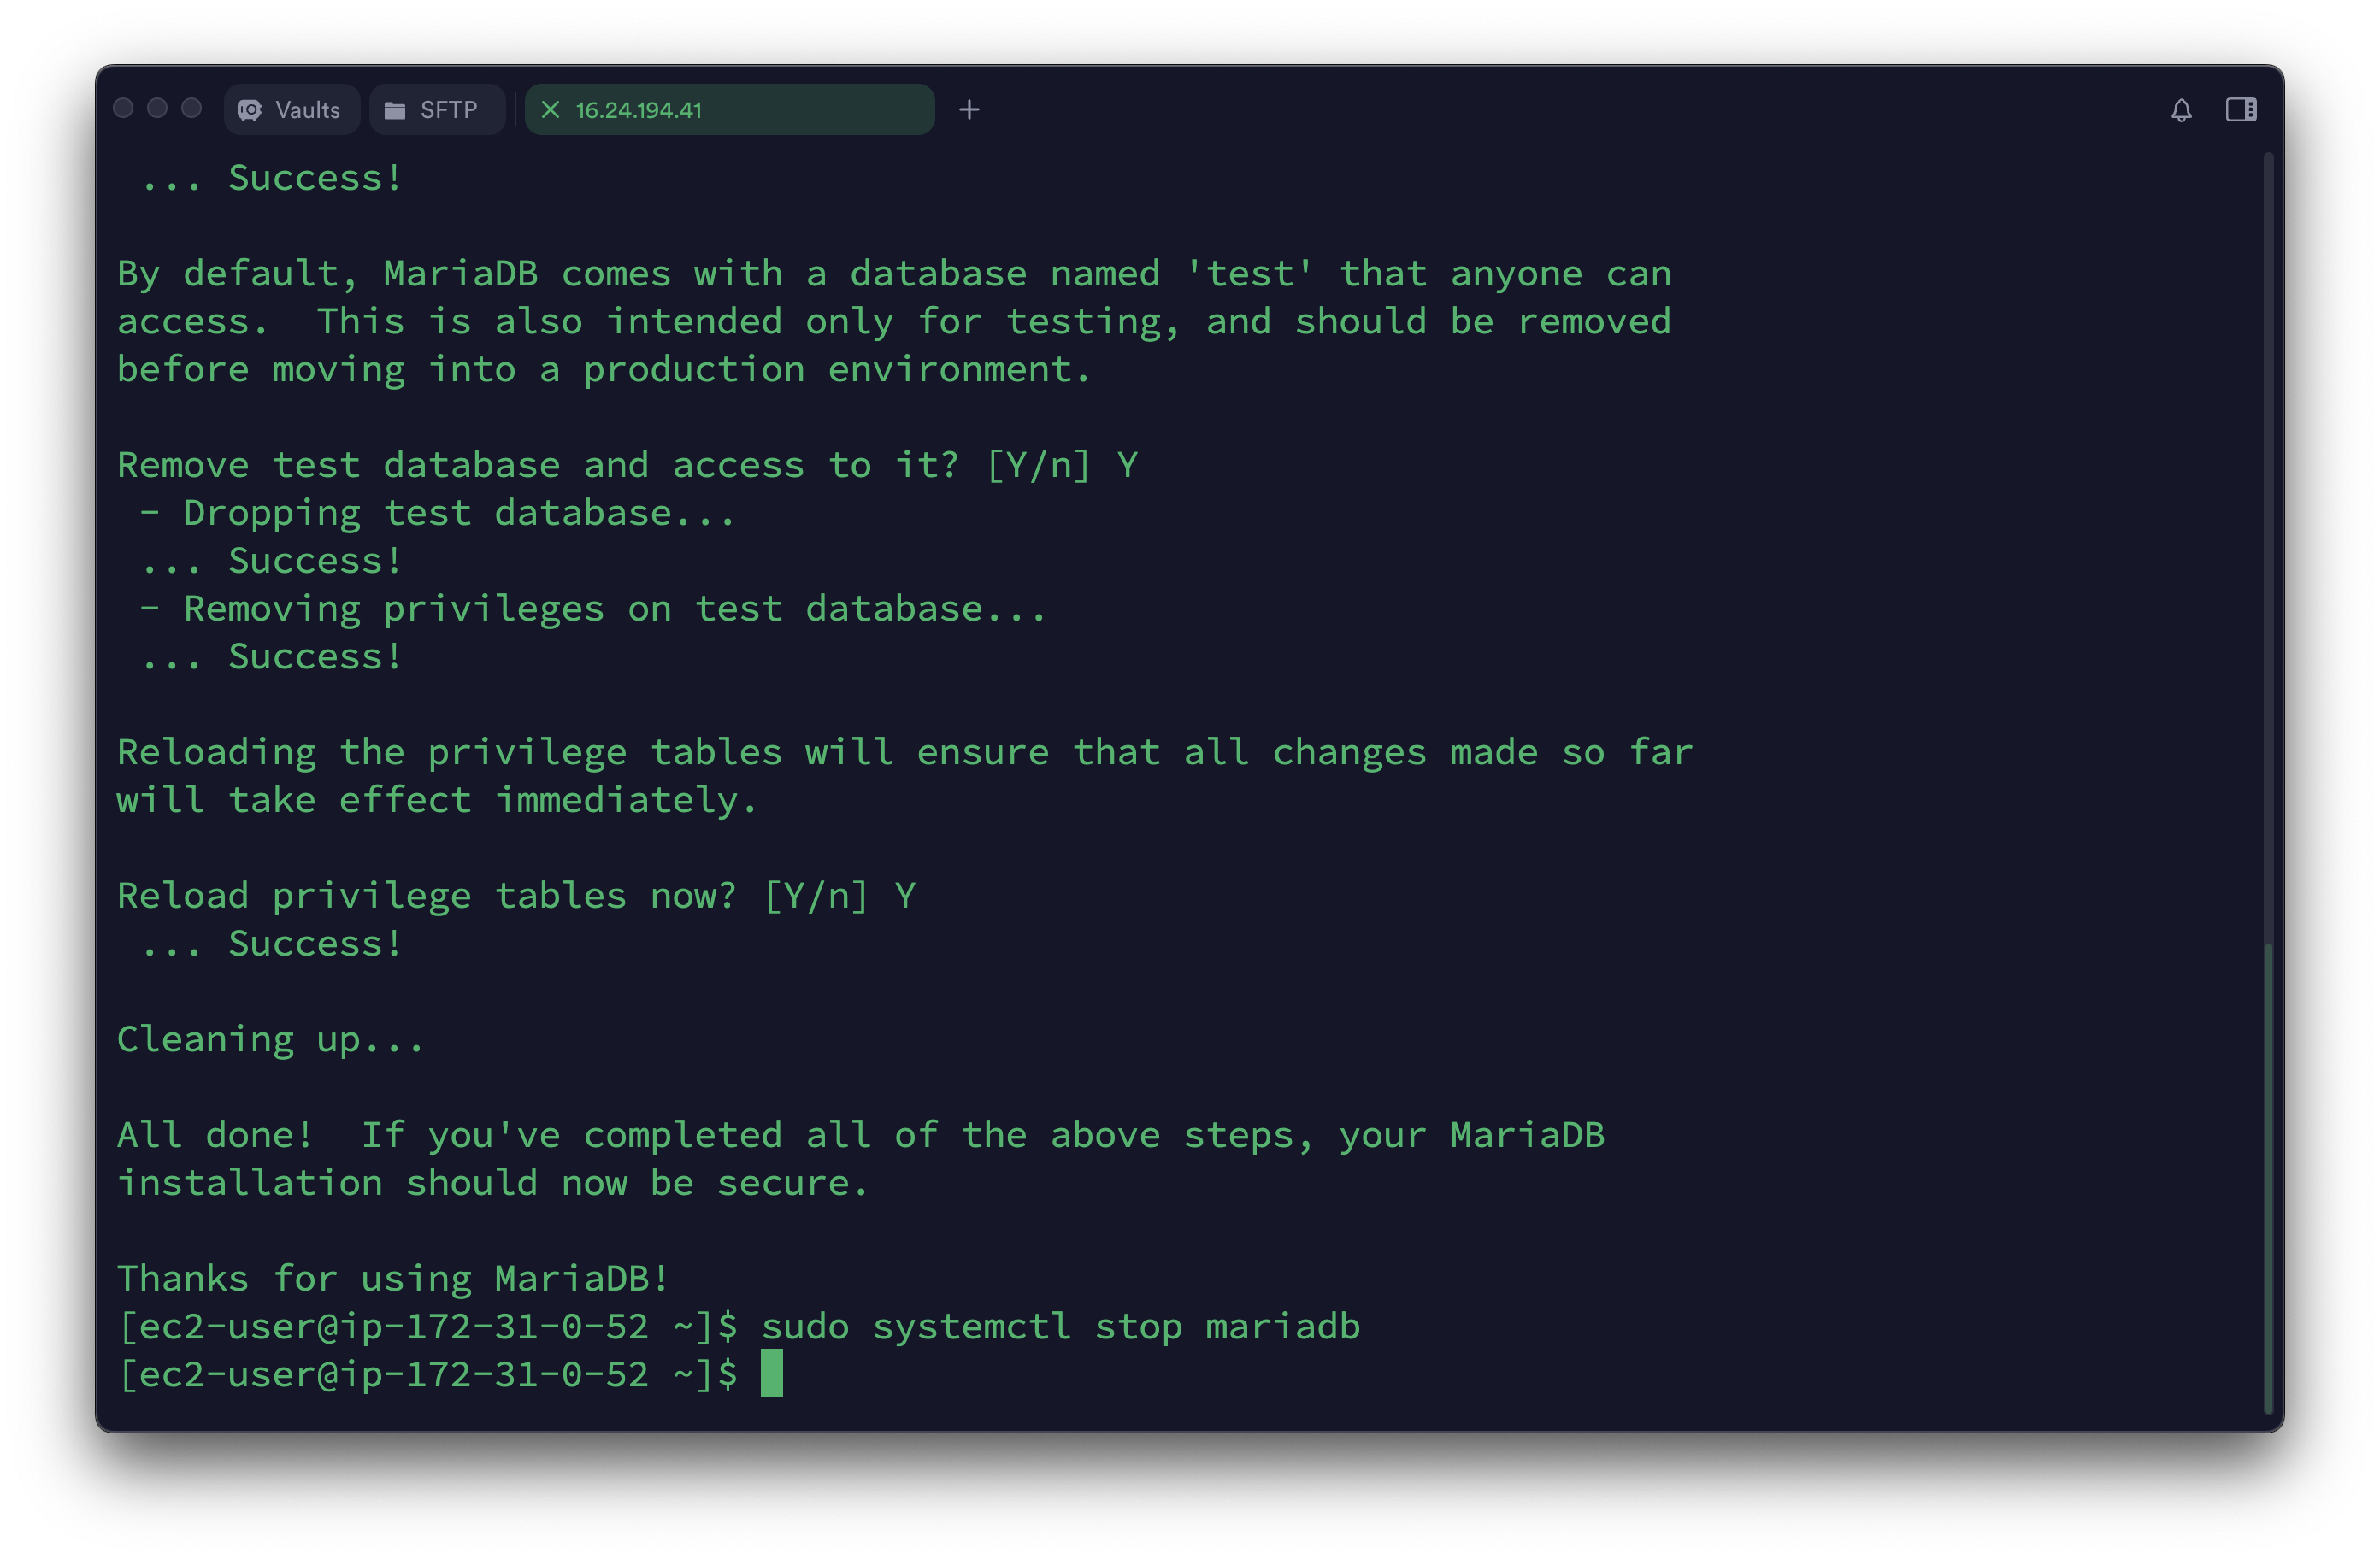
\includegraphics[width=0.95\textwidth]{lamp-server-4.png}
    \caption{LAMP Web Server - MariaDB Secure Setup}
    \label{fig:lamp4}
\end{figure}

\newpage

\section{Part F: Connect to EC2 Linux Instance using Termius on Mac or Windows}

\begin{figure}[H]
    \centering
    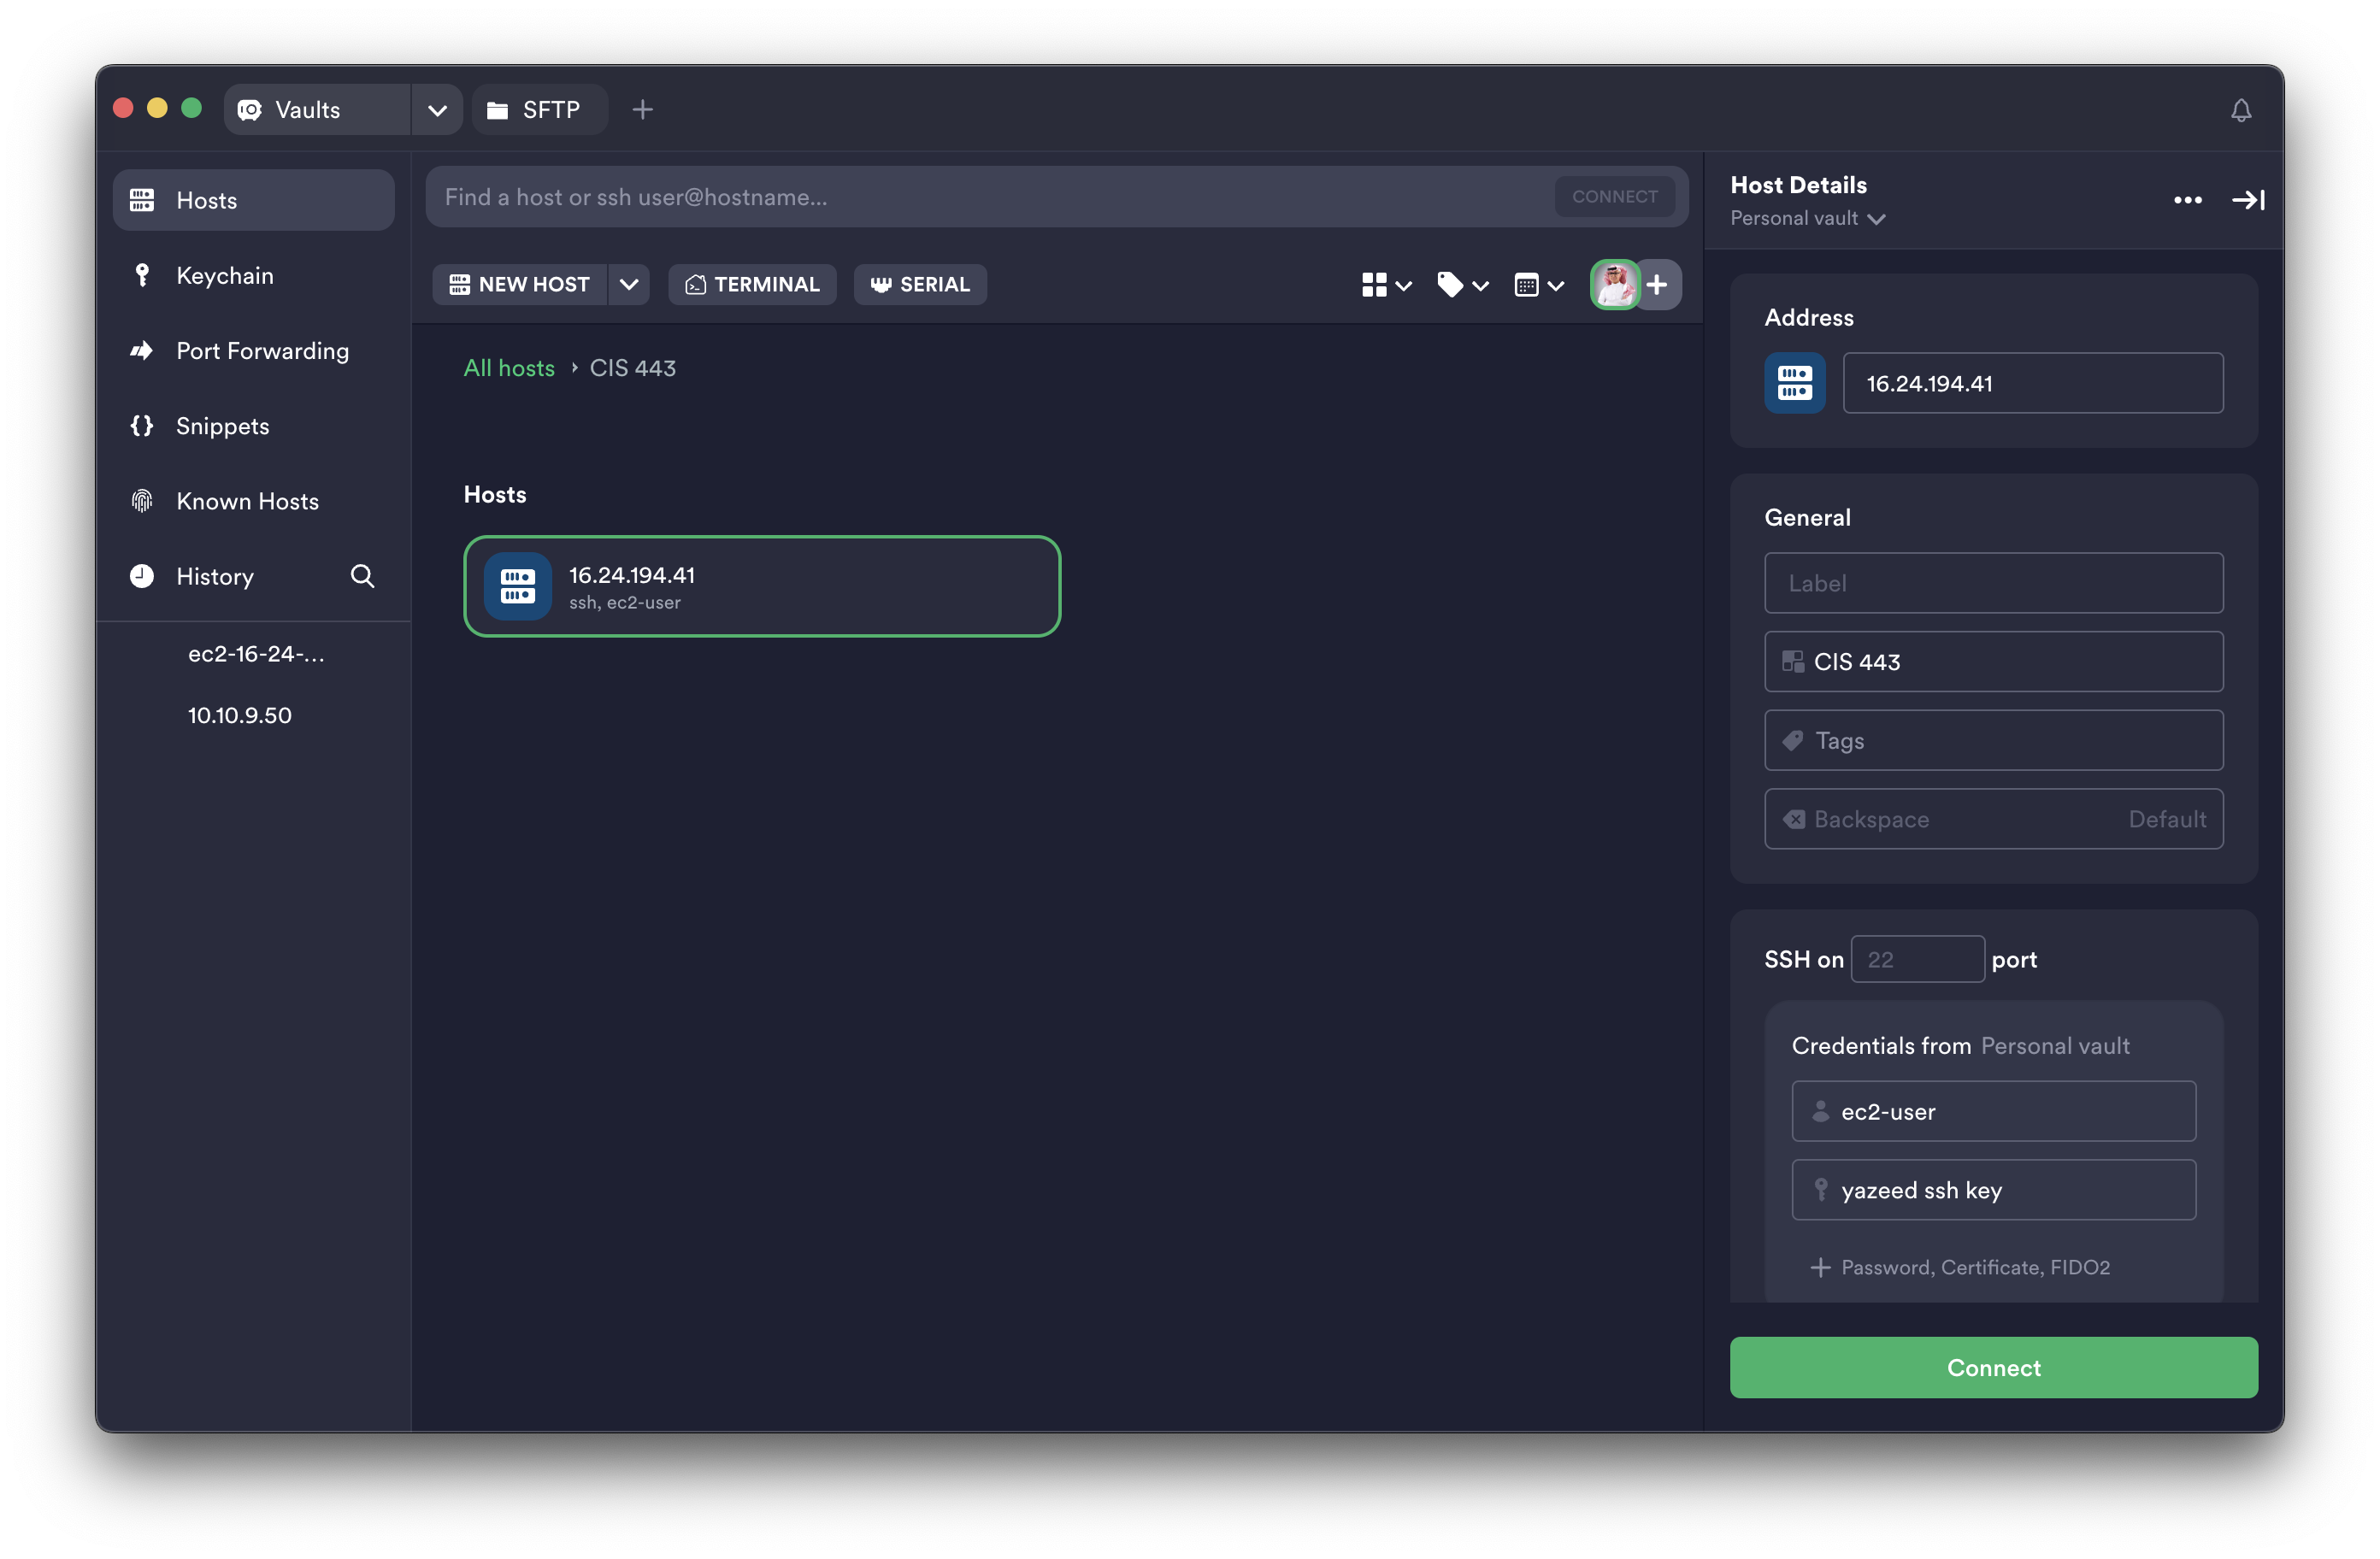
\includegraphics[width=0.95\textwidth]{termius-1.png}
    \caption{Termius SSH Connection Configuration}
    \label{fig:termius1}
\end{figure}

\begin{figure}[H]
    \centering
    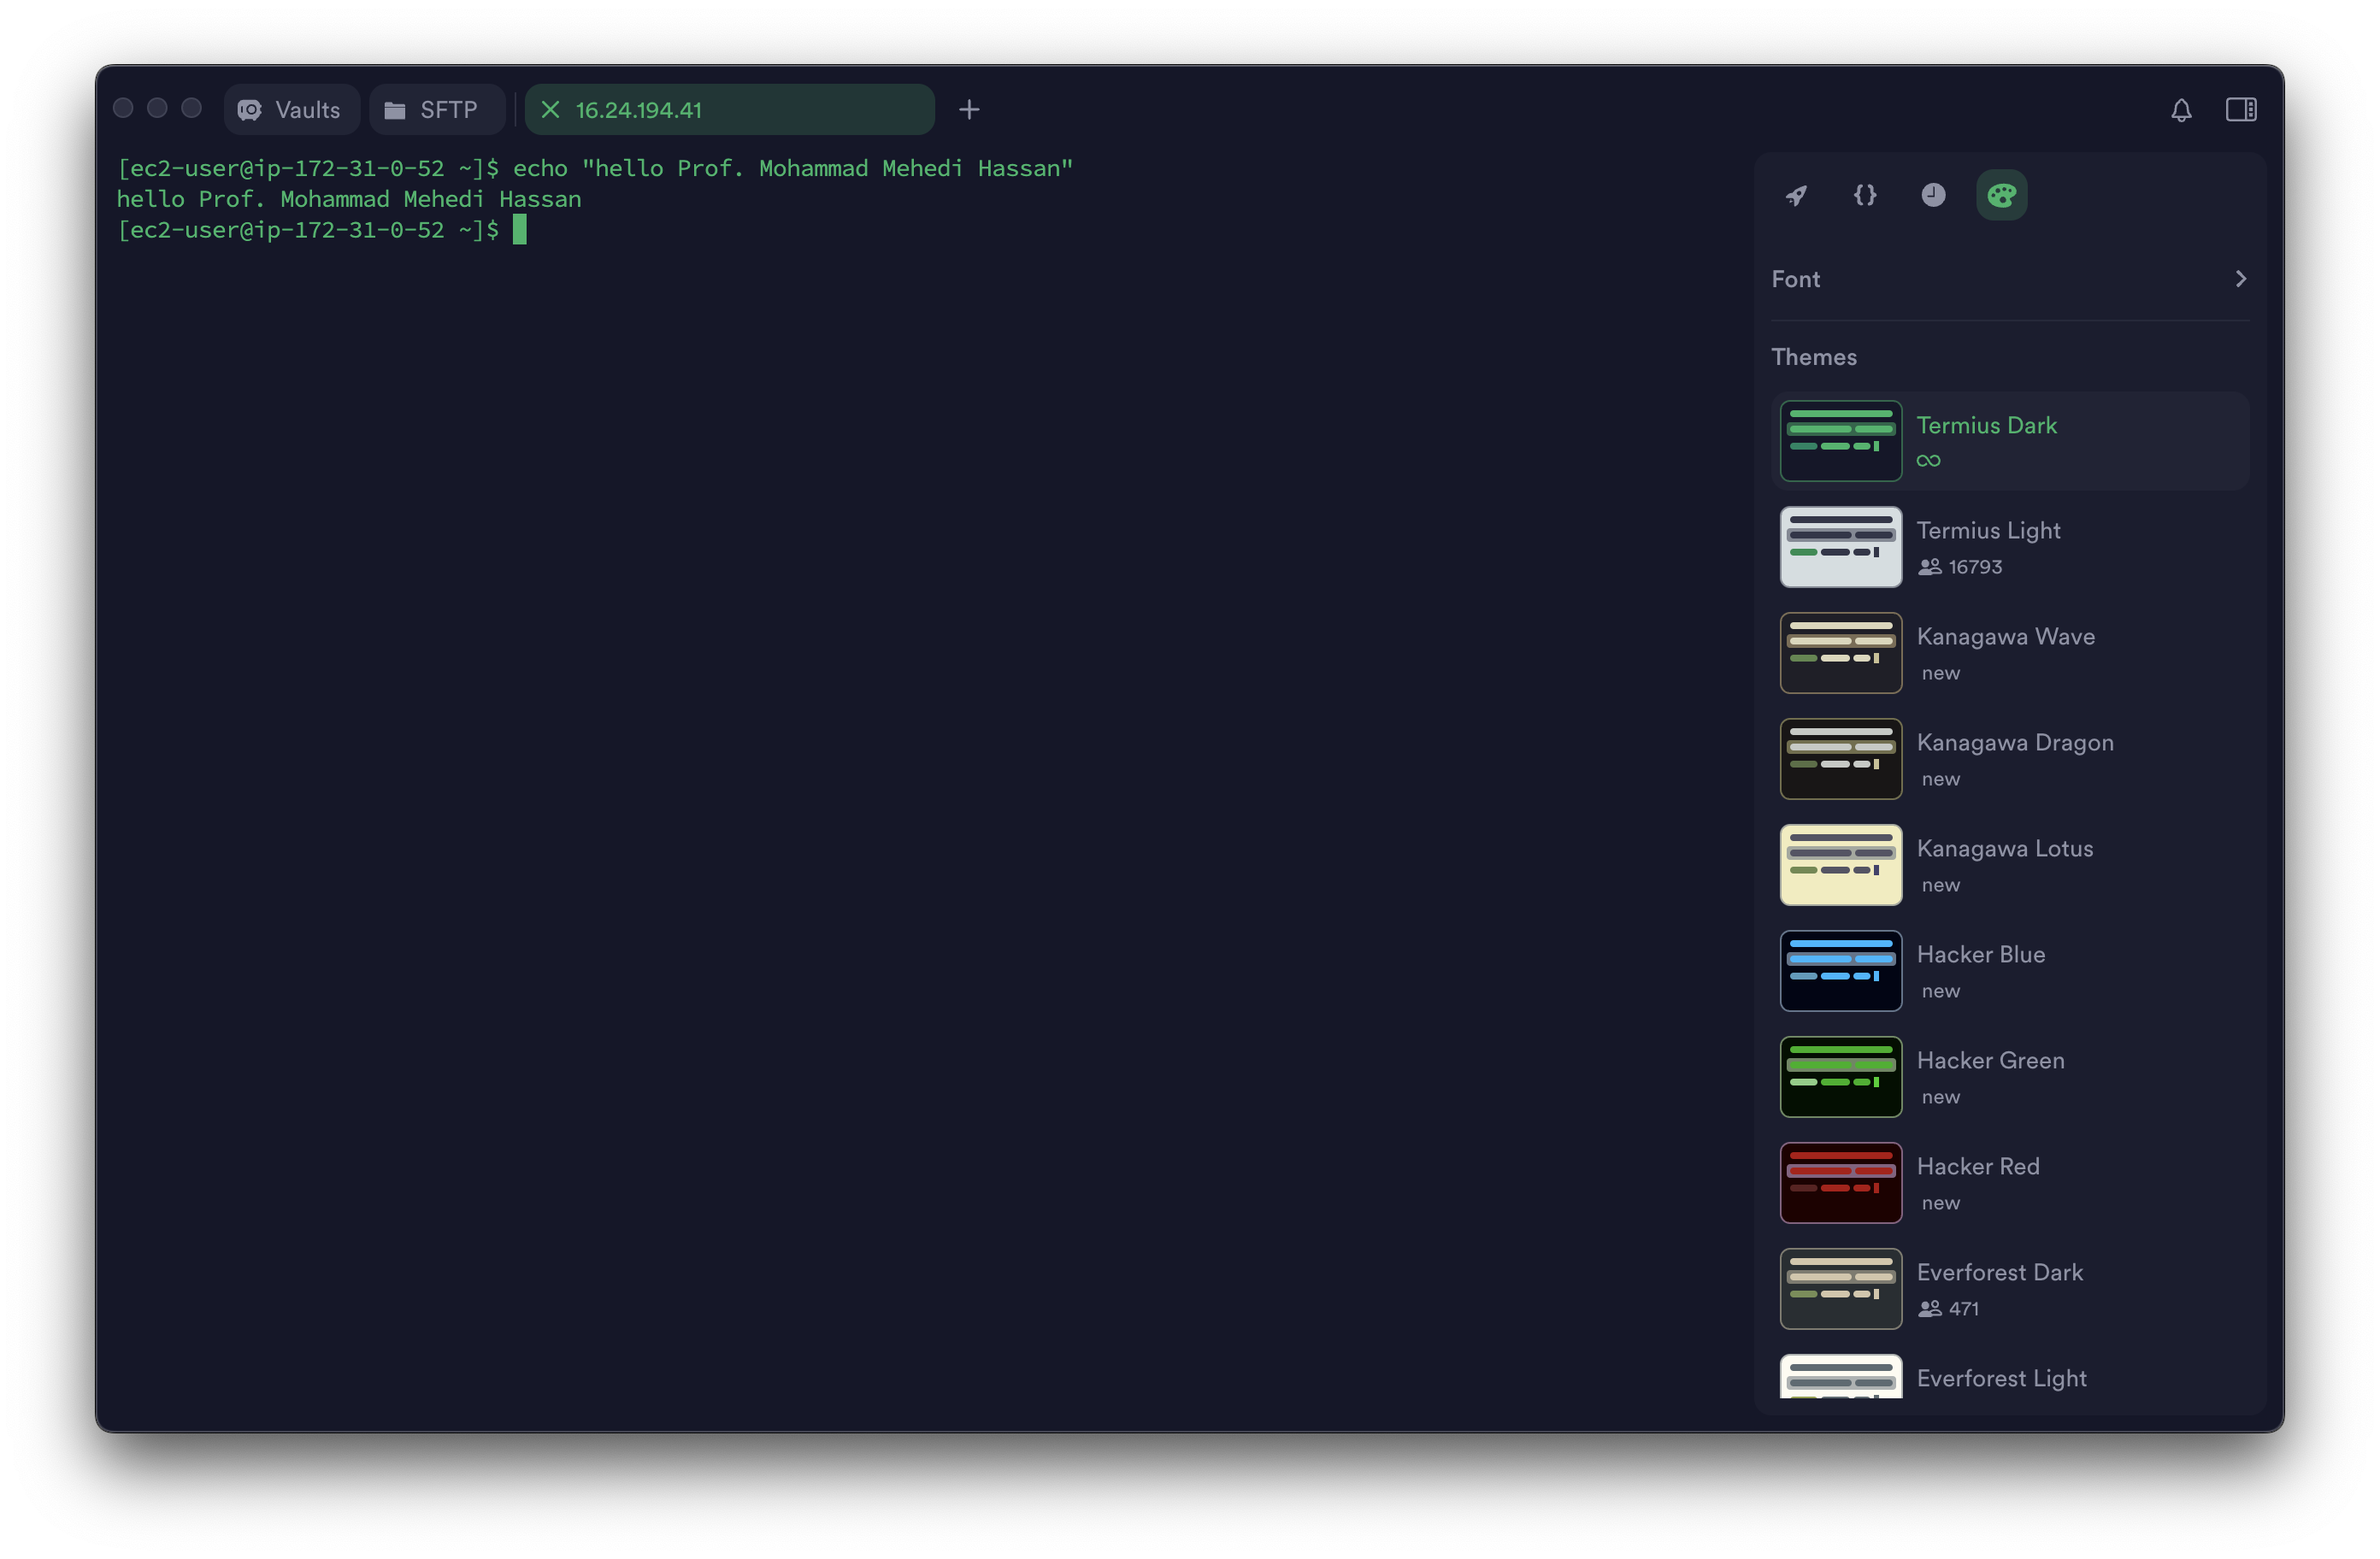
\includegraphics[width=0.95\textwidth]{termius-2.png}
    \caption{Termius SSH Connected - Saying Hello to Professor}
    \label{fig:termius2}
\end{figure}

\end{document}
